\chapter{Results}\label{ch:results}
In this chapter, a simulation of the northern part of Fredericia will be conducted. Furthermore, the results of the simulation will be shown.
\fxnote{stryg sætning ovenfor og start med at goal er at bekræfte at simuleringen virker}

The goal of this simulation is to simulate a daily flow in the northern part of Fredericia, where the disturbance can be seen on the input to the WWTP. To do so the simulation model explained in chapter \ref{ch:simulation} is utilized. The pump station, illustrated with the blue solid circle in figure \ref{fig:kloakgrid_simplified}, is not included in this simulation, as it will smooth the flow from that station down to the WWTP, thus there will not be any variation in the flow into the WWTP. To generate the disturbances from the residential and industrial zones, shown in figure \ref{fig:kloakgrid_simplified}, the flow profiles in appendix \ref{app:flow_profiles} is used. These disturbance models are not simulated from the zones into the main sewer line but are directly added on the main sewer line, therefore the results are expected to have higher peaks, as these models are not attenuated, as they would have been if they were simulated from the zones. It has been chosen to only use the disturbance from the brewery and bottling plant, as the data from the refinery is not accessible. The disturbance from the brewery and bottling plant is shown in figure \ref{fig:flow_profile_industry}. The pipe specifications for this simulation can be seen in table \ref{tab:pipe_data_nonlinear_linear_testv2}.  
\begin{table}[H]
\centering
\begin{tabular}{|c|c|c|c|c|c|c|c|}
\hline
	\rowcolor[HTML]{9B9B9B} 
\begin{tabular}[c]{@{}c@{}}Component\\ number\end{tabular} & Length {[}m{]} & Sections & Dx {[}m{]} & $S_b$     & d {[}m{]} & $\theta$ & \begin{tabular}[c]{@{}c@{}}$Q_f $\\  {[}$m^3/s${]}\end{tabular} \\ \hline
1                                                          & 700            & 35       & 20         & 0,003  & 0,9       & 0,65     & 0,972                                                                          \\ \hline
3                                                          & 303            & 15       & 20,2       & 0,003  & 0,9       & 0,65     & 0,972                                                                          \\ \hline
4                                                          & 27             & 1        & 13,5       & 0,003  & 1         & 0,65     & 1,284                                                                          \\ \hline
5                                                          & 155            & 8        & 19,4       & 0,0041 & 1         & 0,65     & 1,50                                                                           \\ \hline
6                                                          & 295            & 14       & 21         & 0,0122 & 0,8       & 0,65     & 1,438                                                                          \\ \hline
7                                                          & 318            & 15       & 21,2       & 0,0053 & 0,9       & 0,65     & 1,293                                                                          \\ \hline
8                                                          & 110            & 5        & 22         & 0,0036 & 0,9       & 0,65     & 1,066                                                                          \\ \hline
9                                                          & 38             & 2        & 19         & 0,0024 & 1         & 0,65     & 1,149                                                                          \\ \hline
10                                                         & 665            & 30       & 22,2       & 0,003  & 1         & 0,65     & 1,284                                                                          \\ \hline
11                                                         & 155            & 7        & 22,1       & 0,0008 & 1         & 0,65     & 0,663                                                                          \\ \hline
12                                                         & 955            & 47       & 20,3       & 0,0029 & 1,2       & 0,65     & 2,041                                                                          \\ \hline
13                                                         & 304            & 15       & 20,3       & 0,003  & 1,2       & 0,65     & 2,076                                                                          \\ \hline
14                                                         & 116            & 5        & 23,2       & 0,0021 & 1,2       & 0,65     & 1,737                                                                          \\ \hline
15                                                         & 283            & 12       & 23,6       & 0,0017 & 1,4       & 0,65     & 2,346                                                                          \\ \hline
16                                                         & 31             & 2        & 15,5       & 0,0019 & 1,4       & 0,65     & 2,480                                                                          \\ \hline
17                                                         & 125            & 6        & 20,8       & 0,0021 & 1,6       & 0,65     & 3,707                                                                          \\ \hline
18                                                         & 94             & 4        & 23,5       & 0,0013 & 1,5       & 0,65     & 2,461                                                                          \\ \hline
19                                                         & 360            & 18       & 20         & 0,0046 & 1,6       & 0,65     & 5,487                                                                          \\ \hline
20                                                         & 736            & 38       & 19,4         & 0,0012 & 1,6       & 0,65     & 2,802                                                                          \\ \hline
\end{tabular}
\caption{The specification of the pipes for in the simulation.}
\label{tab:pipe_data_nonlinear_linear_testv2}
\end{table}

The tank specification can be seen in table \ref{tab:tank_data_nonlinear_linear_testv2}.

\begin{table}[H]
\centering
\begin{tabular}{|c|c|}
\hline
\begin{tabular}[c]{@{}c@{}}Part\end{tabular} & 2 (Tank)  \\ \hline
Size $[m^3]$                                              & 90 \\ \hline
Height {[}m{]}                                             & 10 \\ \hline
Area {[}$m^2$                                              & 9  \\ \hline
\end{tabular}
\caption{The tank specification for the simulation. }
\label{tab:tank_data_nonlinear_linear_testv2}
\end{table}

Furthermore, table \ref{tab:system_setup_nonlinear_linear_testv2} shows the system setup.

\begin{table}[H]
\centering
\begin{tabular}{|c|c|c|}
\hline
	\rowcolor[HTML]{9B9B9B} 
Type  & Component & Sections \\ \hline
Pipe  & 1         & 35       \\ \hline
Tank  & 1         & 1        \\ \hline
Pipe  & 18        & 227      \\ \hline
Total & 20        & 263      \\ \hline
\end{tabular}
\caption{The system setup.}
\label{tab:system_setup_nonlinear_linear_testv2}
\end{table}

Where the first component in the simulated sewer network is a pipe followed by a tank and hereafter 18 pipes follows. The first pipe and the tank have been added to the original sewer network shown in figure \ref{fig:sewer_line_diagram}. The first pipe goes from the larger industrial area down to the main sewer line showed with a black circle in figure \ref{fig:kloakgrid_simplified}, where the tank is placed as well. The reason for placing the tank there is, that the idea would have been to smoothen the wastewater coming from the larger industry. Furthermore, the pipe is placed, as the MPC could have used it for prediction, as it would be able to measure the disturbance going into the pipe at the industry, and thereby use it in the predictive model to calculate the most optimal control output to the pump. However, as this is not possible, due to the MPC controller is not able to keep a flow output, where the flow variations are kept to a minimum, and as the prediction horizon is limited due to non-convexity as explained in section \ref{se:model_predictive_control}. Therefore in the simulation, the tank will just transfer wastewater from the previous pipe to the pipe after the tank. 

Several simulations were conducted to find the must optimal $\Delta t$ as explained in section \ref{subse:stability_and_precision}. As the pipes are split into different sections and as the average flow height is also different from pipe to pipe, the Courant number variates from pipe to pipe. Thus it is therefore difficult to tune so all pipes have the must optimal Courant number. However, it was found that a $\Delta t = 20$, with the given $\Delta x$ shown in table \ref{tab:pipe_data_nonlinear_linear_testv2}, gave the most realistic outcome, as values lower resulted in an output where some distortion was visible.

In figure \ref{fig:simulation_output_first} the output of a simulation across two days are shown. 

\begin{figure}[H]
\centering
% This file was created by matlab2tikz.
%
%The latest updates can be retrieved from
%  http://www.mathworks.com/matlabcentral/fileexchange/22022-matlab2tikz-matlab2tikz
%where you can also make suggestions and rate matlab2tikz.
%
\definecolor{mycolor1}{rgb}{0.00000,0.44700,0.74100}%
%
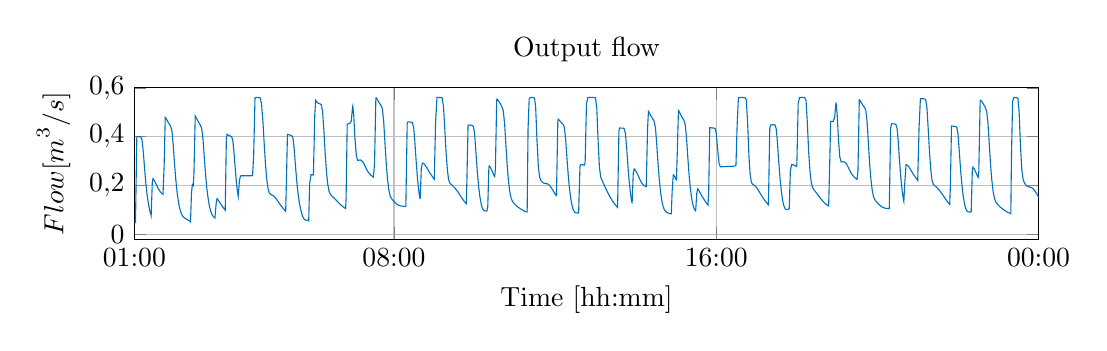
\begin{tikzpicture}

\begin{axis}[%
width=4.521in,
/pgf/number format/1000 sep={.},/pgf/number format/use comma,
height=.7566in,
at={(2.6in,1.103in)},
scale only axis,
scaled x ticks = false,
xmin=5600,
xmax=86401,
xtick={5600,28801,57601,86401,115201,144001,172801},
xticklabels={{01:00},{08:00},{16:00},{00:00},{08:00},{16:00},{00:00},{},{},{}},
xlabel={Time [hh:mm]},
xmajorgrids,
title={Output flow},
ymin=-0.02,
ymax=0.6,
ylabel={$\text{Flow [m}^\text{3}\text{/s]}$},
ymajorgrids,
axis background/.style={fill=white}
]
\addplot [color=mycolor1,solid,forget plot]
  table[row sep=crcr]{%
1	0.0499998870943314\\
21	0.0499999013940726\\
161	0.0499999013424687\\
241	0.0499999013424665\\
341	0.0499999013424741\\
361	0.0499999013423775\\
481	0.0499999011049527\\
561	0.0499998343524527\\
581	0.0500000105656178\\
661	0.0499932182427766\\
701	0.0500437389169566\\
801	0.0473425725067948\\
821	0.052294741748566\\
921	0.13776319907254\\
941	0.133556584111519\\
1061	0.0947162420866767\\
1181	0.0687509896264422\\
1281	0.056843072104176\\
1401	0.0511734456235062\\
1521	0.0501005852471543\\
1641	0.0500047310509262\\
1761	0.0500001279015879\\
1861	0.0499999934879035\\
1941	0.0499999893297788\\
1981	0.0499999899512486\\
2061	0.049999992212563\\
2101	0.0499999918564569\\
2221	0.0499999897632484\\
2241	0.0499999895505436\\
2301	0.0499999902282342\\
2341	0.0499999898377998\\
2441	0.0499999885300658\\
2561	0.0499999890736424\\
2661	0.0499999891936399\\
2781	0.0499999801985208\\
2801	0.0500000167031963\\
2901	0.0500080106730932\\
2921	0.0499659483298955\\
3001	0.0460373492550347\\
3021	0.0649265808451458\\
3141	0.39987471224319\\
3241	0.399999964023972\\
3261	0.399999960475198\\
3381	0.399983812272385\\
3501	0.398370893372803\\
3601	0.382633671255406\\
3721	0.325548916875015\\
3841	0.254124602402494\\
3961	0.193575077309604\\
4081	0.147660897947906\\
4201	0.113902683917788\\
4301	0.0929105561761499\\
4421	0.0742960498494567\\
4541	0.0615252825749841\\
4661	0.053981007385052\\
4781	0.0508535727770067\\
4881	0.0501576222411396\\
5001	0.0500133438776687\\
5121	0.0500007309361146\\
5241	0.0500000168635719\\
5361	0.0499999888871301\\
5461	0.049999992410248\\
5541	0.0500000914733501\\
5581	0.0499985218150507\\
5681	0.0514415462390281\\
5701	0.046037344847944\\
5821	0.399290873297494\\
5941	0.399999974821901\\
6041	0.399997705197\\
6161	0.39956558757164\\
6281	0.388038902151423\\
6401	0.337171656822856\\
6521	0.265587425358579\\
6621	0.212085854215094\\
6741	0.161459520807655\\
6861	0.123997721026595\\
6981	0.0966689341906472\\
7101	0.0760256189325569\\
7201	0.208973210270145\\
7261	0.228026620985395\\
7321	0.225314562793841\\
7441	0.215508125874751\\
7561	0.204239805785136\\
7681	0.192877362755504\\
7801	0.182479057229205\\
7901	0.175181868548256\\
8021	0.168656756218424\\
8141	0.164683176784175\\
8161	0.164315181527722\\
8261	0.280119778842287\\
8361	0.479269340507649\\
8381	0.478423213880455\\
8481	0.470357192358967\\
8601	0.460766826304416\\
8721	0.451836607552887\\
8841	0.443055265656047\\
8961	0.422197990405858\\
9061	0.37390035954862\\
9181	0.295157112154761\\
9301	0.224859390919363\\
9421	0.171224423115168\\
9541	0.132277730995904\\
9641	0.108761268423419\\
9761	0.0892027105991645\\
9881	0.0773595757394141\\
10001	0.070651641952351\\
10121	0.0661775713580224\\
10221	0.0630510193971066\\
10341	0.0597071439387406\\
10461	0.0567949034269938\\
10561	0.0546243491913301\\
10621	0.0512695775424264\\
10701	0.166409800922163\\
10781	0.20357968780827\\
10861	0.199434615905679\\
10921	0.241765963227962\\
11041	0.48473586623314\\
11161	0.474852146426293\\
11281	0.464220664039805\\
11401	0.454578861388125\\
11501	0.447112455841071\\
11621	0.433255957346399\\
11741	0.386075691118731\\
11861	0.308345272313094\\
11981	0.235484355477573\\
12081	0.18735247881565\\
12201	0.143880266060621\\
12321	0.112972942133323\\
12441	0.0920062329118672\\
12561	0.0790804471172134\\
12661	0.0727288362552134\\
12781	0.0675375309217554\\
12801	0.0667206908995505\\
12901	0.121703103554366\\
12981	0.145928679109392\\
13021	0.145166237385415\\
13141	0.136908113729362\\
13241	0.129565327241128\\
13361	0.12112771008752\\
13481	0.113192433438512\\
13601	0.105793149611232\\
13721	0.0991507389943454\\
13821	0.390410622014673\\
13881	0.40986305875768\\
13941	0.408215281082961\\
14061	0.404964079106553\\
14181	0.402566418031675\\
14301	0.399454380267989\\
14401	0.383039216576279\\
14521	0.325637895722135\\
14641	0.254149031848295\\
14761	0.193703509990082\\
14881	0.155368306478837\\
15001	0.224542189947494\\
15101	0.239674727152886\\
15221	0.24000048597446\\
15341	0.240000941023506\\
15461	0.240003221660315\\
15581	0.240006345646753\\
15681	0.240010026513983\\
15801	0.240016079028851\\
15921	0.240038886655287\\
16041	0.240074628249919\\
16161	0.240583491162464\\
16261	0.321307597300039\\
16381	0.559381841100921\\
16501	0.560519913549994\\
16561	0.560519925972796\\
16621	0.56051992245332\\
16741	0.560505572022059\\
16841	0.559092679688636\\
16961	0.535704546442858\\
17081	0.469726208449453\\
17201	0.372386595288142\\
17321	0.284358605955451\\
17421	0.229868633082668\\
17541	0.188124170943587\\
17661	0.169553384083396\\
17781	0.163596333962921\\
17901	0.160813386913845\\
18001	0.158372439794375\\
18121	0.153898437368369\\
18241	0.147573864628597\\
18361	0.14006192436348\\
18481	0.132082854268486\\
18601	0.124128312760278\\
18701	0.117703671201611\\
18821	0.110361752925528\\
18941	0.103480438748526\\
19061	0.0970784182953347\\
19121	0.0940665657039142\\
19181	0.202227299454863\\
19281	0.409784435964215\\
19401	0.407779361361554\\
19521	0.406324765698657\\
19641	0.405518896796074\\
19761	0.396984192809524\\
19861	0.361411317224881\\
19981	0.290581413667561\\
20101	0.222636106333771\\
20221	0.169415715568773\\
20341	0.130021149464464\\
20441	0.105550490648065\\
20561	0.0839453600796147\\
20681	0.0692626520300541\\
20801	0.0608734279665841\\
20921	0.0578654658902276\\
21001	0.0575846925747079\\
21021	0.0576113257709016\\
21141	0.0582847199034818\\
21181	0.0559457131457851\\
21261	0.206468872576803\\
21381	0.244991184003057\\
21501	0.243871395987469\\
21581	0.242763523702759\\
21601	0.243844129628598\\
21721	0.48908138787583\\
21801	0.54901447010447\\
21841	0.546561373522925\\
21961	0.53947750890687\\
22081	0.535939544909621\\
22201	0.534371148629519\\
22301	0.531376482200409\\
22421	0.504216543185119\\
22541	0.421895433415668\\
22661	0.325651681647413\\
22781	0.249560969568209\\
22881	0.205689252233754\\
23001	0.175692296616087\\
23121	0.163596623026188\\
23241	0.157486158404102\\
23361	0.152335457313697\\
23461	0.14803088888763\\
23581	0.142556419278954\\
23701	0.136823291250834\\
23821	0.131050808584863\\
23941	0.125446582725683\\
24041	0.121002035879095\\
24161	0.116027968254653\\
24281	0.111515660096113\\
24401	0.10753397692969\\
24481	0.105546274424128\\
24521	0.147959018171277\\
24621	0.450998540540225\\
24741	0.453497028462156\\
24861	0.454805459366708\\
24981	0.463709456669894\\
25101	0.521501979309344\\
25121	0.525633961984792\\
25201	0.489950057491466\\
25321	0.387119861488875\\
25441	0.320004104853808\\
25561	0.302590046856107\\
25581	0.302486129273871\\
25681	0.303953837704066\\
25761	0.30458675885655\\
25801	0.304452172549737\\
25901	0.302450965268469\\
26021	0.29627627314596\\
26141	0.286497848707108\\
26261	0.275044058907798\\
26381	0.264103064630063\\
26481	0.256418752796677\\
26601	0.249082827305834\\
26721	0.243082254402397\\
26841	0.237997187314841\\
26961	0.234446373563116\\
27061	0.286583479033951\\
27181	0.558179867960004\\
27201	0.559466573038734\\
27301	0.553966955818124\\
27421	0.542471425683814\\
27541	0.534445785404008\\
27641	0.528269213570689\\
27761	0.515323411296657\\
27881	0.462753805460587\\
28001	0.369443460472972\\
28121	0.282092335026993\\
28221	0.226611748143478\\
28341	0.181418486469469\\
28461	0.157290800061398\\
28581	0.14645019607375\\
28701	0.139490911364906\\
28801	0.134398881210367\\
28921	0.128930745444523\\
29041	0.12429008015969\\
29161	0.120637519265873\\
29281	0.118066670808058\\
29401	0.116461543711271\\
29501	0.115639911896372\\
29621	0.114978189452391\\
29741	0.114445529911649\\
29841	0.114080220104003\\
29861	0.11458782154081\\
29981	0.453993741566293\\
30041	0.460896204122244\\
30081	0.46080182975558\\
30201	0.460324978053137\\
30321	0.459845483667925\\
30441	0.458362071337009\\
30561	0.438012442410335\\
30661	0.383537016101309\\
30781	0.299937568944189\\
30901	0.228316855601251\\
31021	0.175285208624054\\
31121	0.146550603859365\\
31141	0.146707741818999\\
31241	0.268673640008559\\
31341	0.292440612392119\\
31361	0.292233270390211\\
31481	0.288649838567375\\
31601	0.282234107570229\\
31721	0.273431509339884\\
31821	0.265400379573232\\
31941	0.256255816271418\\
32061	0.247940021627467\\
32181	0.239749875734644\\
32301	0.231339441297898\\
32401	0.225710685229866\\
32521	0.460798569658897\\
32641	0.56047984402034\\
32761	0.560519925737205\\
32801	0.560519926277395\\
32881	0.560519923039668\\
33001	0.560507866583523\\
33101	0.559051235293447\\
33221	0.526385949827707\\
33341	0.432500247856804\\
33461	0.333009253847885\\
33581	0.260096627074745\\
33681	0.224704607721136\\
33801	0.209095290101304\\
33921	0.204230643411461\\
34041	0.199320034316727\\
34161	0.193751416163673\\
34261	0.18871775381063\\
34381	0.18196902997487\\
34501	0.174311792965989\\
34621	0.166025134280847\\
34741	0.157536417277073\\
34841	0.150574029065654\\
34961	0.14256633356875\\
35081	0.135039059098928\\
35201	0.128059442983278\\
35261	0.125451644802619\\
35321	0.230135460421078\\
35421	0.4478352243038\\
35441	0.44811407769246\\
35541	0.447450613145434\\
35661	0.446957262215923\\
35781	0.446593293634662\\
35901	0.441780080603704\\
36001	0.41278178542571\\
36121	0.338462603239085\\
36241	0.260150478181944\\
36361	0.197967291173421\\
36481	0.152769195922285\\
36601	0.121970042102117\\
36701	0.106193972693711\\
36821	0.097819190631654\\
36941	0.0959989758867092\\
37061	0.0957053801844505\\
37101	0.0956553614348974\\
37181	0.113265409469438\\
37281	0.27546708649598\\
37321	0.280096449864026\\
37401	0.275532438099317\\
37521	0.264265314403432\\
37641	0.251460981815891\\
37761	0.239122810456788\\
37801	0.236596990821348\\
37861	0.266434107289646\\
37981	0.551530978413165\\
38001	0.553366894967955\\
38101	0.549233148595217\\
38221	0.541480209426706\\
38341	0.531830826374847\\
38441	0.522856806397788\\
38561	0.507402402064433\\
38681	0.457048294383577\\
38801	0.366522104329989\\
38921	0.279888650212083\\
39021	0.223897219150489\\
39141	0.176610806368175\\
39261	0.148869110768447\\
39381	0.135496636647129\\
39501	0.128006977760155\\
39601	0.122986721867837\\
39721	0.117745047929022\\
39841	0.113198016463985\\
39961	0.109124948850733\\
40081	0.105315601982642\\
40201	0.101701052031103\\
40301	0.0988946484461107\\
40421	0.0959264433357454\\
40541	0.0935972699431796\\
40661	0.0920236753078962\\
40701	0.0917356687886722\\
40781	0.43220463385167\\
40881	0.555676985515952\\
41001	0.560518359834559\\
41101	0.560519925922487\\
41121	0.560519925652927\\
41241	0.560517635554838\\
41361	0.558546028197403\\
41461	0.52005279135418\\
41581	0.385148808632191\\
41701	0.276221721187392\\
41821	0.233205396477265\\
41941	0.22007389011969\\
42041	0.214155734029736\\
42161	0.210213903552673\\
42281	0.208691609272782\\
42401	0.208015659259071\\
42521	0.206661202976586\\
42621	0.204015313588869\\
42741	0.198416387077501\\
42861	0.190588980297862\\
42981	0.181573721441432\\
43101	0.172311664912568\\
43201	0.164869198821743\\
43301	0.158651139798747\\
43321	0.160003332587438\\
43441	0.463771592578018\\
43481	0.471956377710797\\
43561	0.468236178306124\\
43681	0.461713294115695\\
43801	0.455596497059955\\
43901	0.450804112342984\\
44021	0.438983053031196\\
44141	0.39018412940568\\
44261	0.310460453382816\\
44381	0.236890785360857\\
44481	0.188738153897592\\
44601	0.145759348791124\\
44721	0.116209868654645\\
44841	0.0982692121178757\\
44961	0.0902437318524036\\
45061	0.088086126211636\\
45181	0.087331519464034\\
45281	0.0871144475971674\\
45301	0.0885815963966644\\
45421	0.279281930159125\\
45501	0.285948268035892\\
45541	0.285809216407709\\
45641	0.284913228365149\\
45761	0.283435988553215\\
45801	0.283136547597756\\
45881	0.29370206001371\\
46001	0.534981321586859\\
46121	0.560515237779656\\
46221	0.560519926068477\\
46261	0.560519926376172\\
46341	0.560519926375083\\
46461	0.560519926374744\\
46581	0.560519925675788\\
46701	0.560517516724411\\
46801	0.559663761127618\\
46921	0.518947118184906\\
47041	0.382155172254226\\
47161	0.273187774934129\\
47281	0.233696144419988\\
47401	0.220306974469749\\
47501	0.210282887955032\\
47621	0.198081366820677\\
47741	0.18610567914611\\
47861	0.174629048774868\\
47981	0.163819561489068\\
48081	0.155391116639335\\
48201	0.145973630555617\\
48321	0.137277098070697\\
48441	0.129280549098135\\
48561	0.12195593910867\\
48661	0.116333243347056\\
48781	0.110280587955104\\
48901	0.423332300404789\\
48961	0.435567061037672\\
49021	0.435400366578331\\
49141	0.43513350456344\\
49241	0.435043968808201\\
49361	0.433837256348174\\
49481	0.413797859649674\\
49601	0.34881207657762\\
49721	0.270645091349867\\
49821	0.215437599934438\\
49941	0.164637794114886\\
50061	0.12994319442829\\
50081	0.129323544894529\\
50181	0.248872365137073\\
50261	0.267899772040847\\
50301	0.266601317851276\\
50401	0.260451596159761\\
50521	0.250208284985492\\
50641	0.238193343690953\\
50761	0.22600576500275\\
50881	0.21501144365242\\
51001	0.206302900013726\\
51101	0.201296063092184\\
51221	0.197689607982404\\
51321	0.195657253277077\\
51341	0.195784009404707\\
51461	0.434817816052366\\
51541	0.503592036774015\\
51581	0.5006528180373\\
51681	0.491969672485302\\
51801	0.482171498369809\\
51921	0.473175550309769\\
52041	0.464046410314519\\
52161	0.438249769014414\\
52261	0.382613739606189\\
52381	0.29910595324709\\
52501	0.227484437081824\\
52621	0.174050703320119\\
52741	0.136521511290123\\
52841	0.115494586556638\\
52961	0.100711625356242\\
53081	0.093643699488286\\
53201	0.0896767346579914\\
53321	0.086893187929286\\
53421	0.0852815606931226\\
53541	0.084116300298909\\
53581	0.0839471479111217\\
53661	0.179415615638797\\
53761	0.24409416212698\\
53781	0.243536752492057\\
53901	0.234438737655142\\
54001	0.224876004595448\\
54041	0.22335472358936\\
54121	0.341067920177562\\
54221	0.507566556159231\\
54241	0.506706542280271\\
54361	0.495476555834209\\
54481	0.484948187716946\\
54601	0.475458239796444\\
54701	0.468063870400456\\
54821	0.451630273922372\\
54941	0.396019003666596\\
55061	0.312748391735757\\
55181	0.238197300904533\\
55281	0.190000573395605\\
55401	0.147526628392676\\
55521	0.119148751974907\\
55641	0.10271149206287\\
55741	0.096975498915427\\
55761	0.0989076799566752\\
55861	0.16865769844101\\
55941	0.186119510987269\\
55981	0.184537579099449\\
56101	0.175040938735739\\
56221	0.164979760883986\\
56341	0.155288591004442\\
56441	0.147631770885687\\
56561	0.138996050623163\\
56681	0.13100227293397\\
56801	0.123631187341319\\
56861	0.120312676919824\\
56921	0.17363089926247\\
57021	0.437059337538002\\
57041	0.437782042398014\\
57141	0.436552375035827\\
57261	0.435648324065427\\
57381	0.435383249270215\\
57501	0.432989578135366\\
57601	0.412354764587192\\
57721	0.350377749978731\\
57841	0.292871839410407\\
57961	0.276224861164604\\
57981	0.276216298585415\\
58081	0.276969842062527\\
58201	0.277115386770552\\
58301	0.277283238333835\\
58421	0.277524533378602\\
58541	0.277784035447082\\
58661	0.278043394583852\\
58781	0.278308666145121\\
58881	0.278541246892564\\
59001	0.278823662037737\\
59121	0.279113927785166\\
59241	0.279414711253556\\
59361	0.283682858152549\\
59461	0.442543679072709\\
59581	0.560315623851274\\
59701	0.560519924418927\\
59781	0.56051992637647\\
59821	0.560519926375083\\
59941	0.560519926346461\\
60041	0.560519921996089\\
60161	0.560487536914551\\
60281	0.551985681212544\\
60401	0.457901983254738\\
60521	0.320211588902623\\
60621	0.248326925148368\\
60741	0.212486786855864\\
60861	0.204248805233014\\
60981	0.201408548430853\\
61101	0.197174908469229\\
61201	0.191813106876852\\
61321	0.183686615220915\\
61441	0.174633812913735\\
61561	0.165408284064894\\
61681	0.156433700029906\\
61801	0.147929655831849\\
61901	0.141280685077476\\
62021	0.133845526337268\\
62141	0.127024779985326\\
62261	0.12114747426953\\
62381	0.434310995881452\\
62461	0.44862995078268\\
62501	0.448613963897731\\
62601	0.448724517146426\\
62721	0.449048793139008\\
62781	0.449171273418054\\
62841	0.448632979292017\\
62961	0.431357950634828\\
63061	0.380248672742966\\
63181	0.298539578230001\\
63301	0.227343583077321\\
63421	0.174052489913761\\
63541	0.13676704330989\\
63641	0.116478805986838\\
63761	0.104273434932821\\
63881	0.101406206123581\\
63921	0.101319095647373\\
64001	0.101475023122766\\
64121	0.10538128605057\\
64221	0.261558948924006\\
64341	0.285416138741256\\
64361	0.285451159479523\\
64461	0.285035573060551\\
64581	0.283276000044435\\
64701	0.279264645059642\\
64761	0.277772752431824\\
64801	0.285705622410285\\
64921	0.537281741958665\\
65041	0.560516283463776\\
65161	0.56051992632738\\
65201	0.560519926375697\\
65281	0.560519926297225\\
65401	0.560519857746322\\
65501	0.560447718328738\\
65621	0.548710871267265\\
65741	0.454096831838203\\
65861	0.334363528136731\\
65981	0.255692401767726\\
66081	0.215441634575985\\
66201	0.191958319017027\\
66321	0.182685826517502\\
66441	0.175872082839274\\
66561	0.168900866046064\\
66661	0.162840514640622\\
66781	0.15545500033445\\
66901	0.148224355100308\\
67021	0.141326215315489\\
67141	0.134918978321645\\
67241	0.130027682716447\\
67361	0.12475999806964\\
67481	0.120283427647202\\
67601	0.116760182085105\\
67641	0.115879979337036\\
67721	0.256906694277138\\
67821	0.462328178781824\\
67941	0.462742467311499\\
68061	0.463229136391895\\
68181	0.479996449086711\\
68301	0.540634292807742\\
68401	0.494671436614675\\
68521	0.386409476375928\\
68641	0.316611148546197\\
68761	0.296624864709725\\
68801	0.296195136717095\\
68881	0.296950957771465\\
68941	0.297296204144505\\
69001	0.297071853615368\\
69101	0.295044151872098\\
69221	0.289165469064049\\
69341	0.279693494347913\\
69461	0.268317008474507\\
69581	0.257124610320087\\
69681	0.249037321708162\\
69801	0.241209546310923\\
69921	0.2349004662421\\
70041	0.229497399493195\\
70161	0.225354030117976\\
70181	0.225059489271662\\
70261	0.259200655208592\\
70381	0.549847034621941\\
70401	0.550882310331099\\
70501	0.543814392214192\\
70621	0.53468062556008\\
70741	0.526626354438835\\
70841	0.520518840063806\\
70961	0.508492942465399\\
71081	0.458885709156494\\
71201	0.367678915054067\\
71321	0.280835008046728\\
71421	0.225082093505229\\
71541	0.17874554050684\\
71661	0.152795946630158\\
71781	0.140899689178609\\
71901	0.133751727076324\\
72001	0.128569837245537\\
72121	0.122900982288641\\
72241	0.117899782713044\\
72361	0.11370937999743\\
72481	0.11047669621739\\
72601	0.108253917208387\\
72701	0.107086173954667\\
72821	0.106244396685782\\
72941	0.105705504850461\\
73061	0.105332967336101\\
73181	0.435946178239638\\
73261	0.453024300871342\\
73281	0.452993182645803\\
73401	0.452643145741346\\
73521	0.452285281378683\\
73641	0.451074937198832\\
73761	0.432700419795512\\
73861	0.380786552315047\\
73981	0.298685805564177\\
74101	0.22740378491374\\
74221	0.174126253302158\\
74341	0.137527670304174\\
74361	0.134237338321971\\
74441	0.207813944879953\\
74561	0.285378186391529\\
74681	0.282741308206488\\
74801	0.276860325385806\\
74921	0.268441499011197\\
75021	0.260531228340002\\
75141	0.251358476916889\\
75261	0.243047767537963\\
75381	0.234991099963782\\
75501	0.22669534135459\\
75601	0.220651866001535\\
75721	0.435682734941586\\
75841	0.555644546524901\\
75861	0.5556579938168\\
75961	0.555532786553423\\
76081	0.555345184989036\\
76201	0.555134531244548\\
76301	0.553070405897535\\
76421	0.52143634234302\\
76541	0.430650361480022\\
76661	0.331737174382703\\
76781	0.258220582010269\\
76881	0.221453052319226\\
77001	0.204370131882797\\
77121	0.199490556820935\\
77241	0.194840612652044\\
77361	0.189447032372619\\
77461	0.18459818792937\\
77581	0.178156275286525\\
77701	0.17082709182546\\
77821	0.162801718838174\\
77941	0.154504652252671\\
78041	0.147651817985528\\
78161	0.139721338607162\\
78281	0.132237289719755\\
78401	0.125268158898425\\
78461	0.122293389503727\\
78521	0.200183883244457\\
78621	0.443371234685954\\
78641	0.44384907080836\\
78741	0.443118174300164\\
78861	0.442576453515615\\
78981	0.442284453908172\\
79101	0.437894496579005\\
79201	0.410266374618955\\
79321	0.337402619298452\\
79441	0.259592450508481\\
79561	0.1974736282187\\
79681	0.152086532284992\\
79801	0.120736618732429\\
79901	0.104045551939936\\
80021	0.0943411879687305\\
80141	0.0918844815760334\\
80261	0.0914814175777137\\
80341	0.0913677029693039\\
80381	0.0933537585439379\\
80481	0.25937975551348\\
80541	0.275622277873239\\
80601	0.27249003978879\\
80721	0.261519038370172\\
80841	0.248802076595153\\
80961	0.236383276945911\\
81001	0.233525034544167\\
81061	0.257458533473377\\
81181	0.54687447664287\\
81201	0.549299988830962\\
81301	0.545439554226405\\
81421	0.537797759572825\\
81541	0.5282779599033\\
81641	0.519364013104925\\
81761	0.504184946635507\\
81881	0.455073866937148\\
82001	0.365589134600443\\
82121	0.279243357391384\\
82221	0.223161675675254\\
82341	0.175385254318035\\
82461	0.146694770515305\\
82581	0.132468523490279\\
82701	0.124594492891463\\
82801	0.119381319389791\\
82921	0.113897384115697\\
83041	0.109107129588899\\
83161	0.104849021773584\\
83281	0.100914675777395\\
83401	0.0971687821357265\\
83501	0.094188773553084\\
83621	0.0909083755439143\\
83741	0.0881201902184991\\
83861	0.0859844112128927\\
83921	0.0850802881804396\\
83981	0.326357451856701\\
84081	0.545637947539441\\
84201	0.560496119485827\\
84321	0.560519924141328\\
84441	0.560511089788814\\
84561	0.556309944537726\\
84661	0.502961791273052\\
84781	0.364224489875436\\
84901	0.265208785570677\\
85021	0.224848732047967\\
85141	0.210318218658298\\
85241	0.203193126166625\\
85361	0.197700042531359\\
85481	0.194910469082314\\
85601	0.193529004029528\\
85721	0.192135105344627\\
85821	0.18997400132247\\
85941	0.185302879917271\\
86061	0.178328731520561\\
86181	0.169791880525794\\
86301	0.160638917604341\\
86401	0.153045543821935\\
86521	0.144709226768709\\
86641	0.419141298934461\\
86701	0.454054707630259\\
86761	0.451394019142469\\
86881	0.444628463516935\\
87001	0.43803930691914\\
87101	0.432783697121007\\
87221	0.422328786617079\\
87341	0.380678943401039\\
87461	0.306273337979366\\
87581	0.234450959559099\\
87681	0.186507531142102\\
87801	0.142889472888738\\
87921	0.111484258449539\\
88041	0.0895771933695757\\
88161	0.0754579521803443\\
88261	0.0686342760780883\\
88381	0.0643654258839812\\
88501	0.0620940168384219\\
88621	0.060777251205792\\
88661	0.0585887035110699\\
88741	0.205268680191705\\
88841	0.251606154284689\\
88961	0.250277814249827\\
89041	0.24924148963148\\
89081	0.250642017017168\\
89201	0.484896319610643\\
89321	0.560490180852446\\
89421	0.560519924769304\\
89481	0.560519926376424\\
89541	0.560519926374993\\
89661	0.560519926102528\\
89781	0.560519449721204\\
89901	0.559752019207538\\
90001	0.535593075519315\\
90121	0.413254622013994\\
90241	0.293326587472733\\
90361	0.232126865500809\\
90481	0.208532880603294\\
90601	0.197146259995847\\
90701	0.188406952078761\\
90821	0.177557602352001\\
90941	0.166559090951186\\
91061	0.155753731952714\\
91181	0.145369082827036\\
91281	0.137155093513777\\
91401	0.127884797755217\\
91521	0.119258801900499\\
91641	0.11127985661749\\
91761	0.103899558227189\\
91861	0.0981894307584928\\
91981	0.0918291888240484\\
92041	0.0887876709313282\\
92101	0.252445263802945\\
92201	0.404365602842541\\
92221	0.404070500301085\\
92341	0.402011327334036\\
92441	0.400942054743135\\
92561	0.399866137788076\\
92681	0.388113869885826\\
92801	0.337183571321159\\
92921	0.265589387610062\\
93021	0.2120865820883\\
93141	0.161459952603468\\
93261	0.123998095758113\\
93381	0.096669304121437\\
93501	0.0760260025863379\\
93601	0.208973714239511\\
93661	0.228026644045997\\
93721	0.225314563541965\\
93841	0.215508125875328\\
93961	0.204239805785136\\
94081	0.192877362755504\\
94201	0.182479057229204\\
94301	0.175181868548256\\
94421	0.168656756218424\\
94541	0.164683176784175\\
94561	0.164315181527722\\
94661	0.280119778842286\\
94761	0.479269340507649\\
94781	0.478423213880455\\
94881	0.470357192358967\\
95001	0.460766826304416\\
95121	0.451836607552887\\
95241	0.443055265656047\\
95361	0.422197990405859\\
95461	0.37390035954862\\
95581	0.295157112154761\\
95701	0.224859390919362\\
95821	0.171224423115168\\
95941	0.132277730995904\\
96041	0.108761268423419\\
96161	0.0892027105991645\\
96281	0.0773595757394139\\
96401	0.070651641952351\\
96521	0.0661775713580222\\
96621	0.0630510193971069\\
96741	0.0597071439387406\\
96861	0.0567949034269939\\
96961	0.05462434919133\\
97021	0.0512695775424262\\
97101	0.166409800922163\\
97181	0.203579687808269\\
97261	0.199434615905679\\
97321	0.241765963227962\\
97441	0.48473586623314\\
97561	0.474852146426293\\
97681	0.464220664039805\\
97801	0.454578861388124\\
97901	0.447112455841071\\
98021	0.433255957346399\\
98141	0.386075691118731\\
98261	0.308345272313094\\
98381	0.235484355477573\\
98481	0.18735247881565\\
98601	0.14388026606062\\
98721	0.112972942133323\\
98841	0.0920062329118677\\
98961	0.0790804471172137\\
99061	0.0727288362552131\\
99181	0.0675375309217557\\
99201	0.0667206908995503\\
99301	0.121703103554366\\
99381	0.145928679109392\\
99421	0.145166237385415\\
99541	0.136908113729361\\
99641	0.129565327241128\\
99761	0.12112771008752\\
99881	0.113192433438513\\
100001	0.105793149611232\\
100121	0.0991507389943453\\
100221	0.390410622014674\\
100281	0.40986305875768\\
100341	0.408215281082961\\
100461	0.404964079106553\\
100581	0.402566418031675\\
100701	0.399454380267989\\
100801	0.383039216576279\\
100921	0.325637895722135\\
101041	0.254149031848295\\
101161	0.193703509990082\\
101281	0.155368306478837\\
101401	0.224542189947494\\
101501	0.239674727152886\\
101621	0.24000048597446\\
101741	0.240000941023506\\
101861	0.240003221660315\\
101981	0.240006345646753\\
102081	0.240010026513983\\
102201	0.240016079028851\\
102321	0.240038886655287\\
102441	0.240074628249919\\
102561	0.240583491162464\\
102661	0.321307597300039\\
102781	0.559381841100921\\
102901	0.560519913549994\\
102961	0.560519925972796\\
103021	0.56051992245332\\
103141	0.560505572022059\\
103241	0.559092679688636\\
103361	0.535704546442858\\
103481	0.469726208449453\\
103601	0.372386595288142\\
103721	0.284358605955451\\
103821	0.229868633082668\\
103941	0.188124170943587\\
104061	0.169553384083396\\
104181	0.163596333962921\\
104301	0.160813386913845\\
104401	0.158372439794375\\
104521	0.153898437368369\\
104641	0.147573864628597\\
104761	0.14006192436348\\
104881	0.132082854268486\\
105001	0.124128312760278\\
105101	0.117703671201611\\
105221	0.110361752925528\\
105341	0.103480438748526\\
105461	0.0970784182953347\\
105521	0.0940665657039142\\
105581	0.202227299454863\\
105681	0.409784435964215\\
105801	0.407779361361554\\
105921	0.406324765698657\\
106041	0.405518896796074\\
106161	0.396984192809524\\
106261	0.361411317224881\\
106381	0.290581413667561\\
106501	0.222636106333771\\
106621	0.169415715568773\\
106741	0.130021149464464\\
106841	0.105550490648065\\
106961	0.0839453600796147\\
107081	0.0692626520300541\\
107201	0.0608734279665841\\
107321	0.0578654658902276\\
107401	0.0575846925747079\\
107421	0.0576113257709016\\
107541	0.0582847199034818\\
107581	0.0559457131457851\\
107661	0.206468872576803\\
107781	0.244991184003057\\
107901	0.243871395987469\\
107981	0.242763523702759\\
108001	0.243844129628598\\
108121	0.48908138787583\\
108201	0.54901447010447\\
108241	0.546561373522925\\
108361	0.53947750890687\\
108481	0.535939544909621\\
108601	0.534371148629519\\
108701	0.531376482200409\\
108821	0.504216543185119\\
108941	0.421895433415668\\
109061	0.325651681647413\\
109181	0.249560969568209\\
109281	0.205689252233754\\
109401	0.175692296616087\\
109521	0.163596623026188\\
109641	0.157486158404102\\
109761	0.152335457313697\\
109861	0.14803088888763\\
109981	0.142556419278954\\
110101	0.136823291250834\\
110221	0.131050808584863\\
110341	0.125446582725683\\
110441	0.121002035879095\\
110561	0.116027968254653\\
110681	0.111515660096113\\
110801	0.10753397692969\\
110881	0.105546274424128\\
110921	0.147959018171277\\
111021	0.450998540540225\\
111141	0.453497028462156\\
111261	0.454805459366708\\
111381	0.463709456669894\\
111501	0.521501979309344\\
111521	0.525633961984792\\
111601	0.489950057491466\\
111721	0.387119861488875\\
111841	0.320004104853808\\
111961	0.302590046856107\\
111981	0.302486129273871\\
112081	0.303953837704066\\
112161	0.30458675885655\\
112201	0.304452172549737\\
112301	0.302450965268469\\
112421	0.29627627314596\\
112541	0.286497848707108\\
112661	0.275044058907798\\
112781	0.264103064630063\\
112881	0.256418752796677\\
113001	0.249082827305834\\
113121	0.243082254402397\\
113241	0.237997187314841\\
113361	0.234446373563116\\
113461	0.286583479033951\\
113581	0.558179867960004\\
113601	0.559466573038734\\
113701	0.553966955818124\\
113821	0.542471425683814\\
113941	0.534445785404008\\
114041	0.528269213570689\\
114161	0.515323411296657\\
114281	0.462753805460587\\
114401	0.369443460472972\\
114521	0.282092335026993\\
114621	0.226611748143478\\
114741	0.181418486469469\\
114861	0.157290800061398\\
114981	0.14645019607375\\
115101	0.139490911364906\\
115201	0.134398881210367\\
115321	0.128930745444523\\
115441	0.12429008015969\\
115561	0.120637519265873\\
115681	0.118066670808058\\
115801	0.116461543711271\\
115901	0.115639911896372\\
116021	0.114978189452391\\
116141	0.114445529911649\\
116241	0.114080220104003\\
116261	0.11458782154081\\
116381	0.453993741566293\\
116441	0.460896204122244\\
116481	0.46080182975558\\
116601	0.460324978053137\\
116721	0.459845483667925\\
116841	0.458362071337009\\
116961	0.438012442410335\\
117061	0.383537016101309\\
117181	0.299937568944189\\
117301	0.228316855601251\\
117421	0.175285208624054\\
117521	0.146550603859365\\
117541	0.146707741818999\\
117641	0.268673640008559\\
117741	0.292440612392119\\
117761	0.292233270390211\\
117881	0.288649838567375\\
118001	0.282234107570229\\
118121	0.273431509339884\\
118221	0.265400379573232\\
118341	0.256255816271418\\
118461	0.247940021627467\\
118581	0.239749875734644\\
118701	0.231339441297898\\
118801	0.225710685229866\\
118921	0.460798569658897\\
119041	0.56047984402034\\
119161	0.560519925737205\\
119201	0.560519926277395\\
119281	0.560519923039668\\
119401	0.560507866583523\\
119501	0.559051235293447\\
119621	0.526385949827707\\
119741	0.432500247856804\\
119861	0.333009253847885\\
119981	0.260096627074745\\
120081	0.224704607721136\\
120201	0.209095290101304\\
120321	0.204230643411461\\
120441	0.199320034316727\\
120561	0.193751416163673\\
120661	0.18871775381063\\
120781	0.18196902997487\\
120901	0.174311792965989\\
121021	0.166025134280847\\
121141	0.157536417277073\\
121241	0.150574029065654\\
121361	0.14256633356875\\
121481	0.135039059098928\\
121601	0.128059442983278\\
121661	0.125451644802619\\
121721	0.230135460421078\\
121821	0.4478352243038\\
121841	0.44811407769246\\
121941	0.447450613145434\\
122061	0.446957262215923\\
122181	0.446593293634662\\
122301	0.441780080603704\\
122401	0.41278178542571\\
122521	0.338462603239085\\
122641	0.260150478181944\\
122761	0.197967291173421\\
122881	0.152769195922285\\
123001	0.121970042102117\\
123101	0.106193972693711\\
123221	0.097819190631654\\
123341	0.0959989758867092\\
123461	0.0957053801844505\\
123501	0.0956553614348974\\
123581	0.113265409469438\\
123681	0.27546708649598\\
123721	0.280096449864026\\
123801	0.275532438099317\\
123921	0.264265314403432\\
124041	0.251460981815891\\
124161	0.239122810456788\\
124201	0.236596990821348\\
124261	0.266434107289646\\
124381	0.551530978413165\\
124401	0.553366894967955\\
124501	0.549233148595217\\
124621	0.541480209426706\\
124741	0.531830826374847\\
124841	0.522856806397788\\
124961	0.507402402064433\\
125081	0.457048294383577\\
125201	0.366522104329989\\
125321	0.279888650212083\\
125421	0.223897219150489\\
125541	0.176610806368175\\
125661	0.148869110768447\\
125781	0.135496636647129\\
125901	0.128006977760155\\
126001	0.122986721867837\\
126121	0.117745047929022\\
126241	0.113198016463985\\
126361	0.109124948850733\\
126481	0.105315601982642\\
126601	0.101701052031103\\
126701	0.0988946484461107\\
126821	0.0959264433357454\\
126941	0.0935972699431796\\
127061	0.0920236753078962\\
127101	0.0917356687886722\\
127181	0.43220463385167\\
127281	0.555676985515952\\
127401	0.560518359834559\\
127501	0.560519925922487\\
127521	0.560519925652927\\
127641	0.560517635554838\\
127761	0.558546028197403\\
127861	0.52005279135418\\
127981	0.385148808632191\\
128101	0.276221721187392\\
128221	0.233205396477265\\
128341	0.22007389011969\\
128441	0.214155734029736\\
128561	0.210213903552673\\
128681	0.208691609272782\\
128801	0.208015659259071\\
128921	0.206661202976586\\
129021	0.204015313588869\\
129141	0.198416387077501\\
129261	0.190588980297862\\
129381	0.181573721441432\\
129501	0.172311664912568\\
129601	0.164869198821743\\
129701	0.158651139798747\\
129721	0.160003332587438\\
129841	0.463771592578018\\
129881	0.471956377710797\\
129961	0.468236178306124\\
130081	0.461713294115695\\
130201	0.455596497059955\\
130301	0.450804112342984\\
130421	0.438983053031196\\
130541	0.39018412940568\\
130661	0.310460453382816\\
130781	0.236890785360857\\
130881	0.188738153897592\\
131001	0.145759348791124\\
131121	0.116209868654645\\
131241	0.0982692121178757\\
131361	0.0902437318524036\\
131461	0.088086126211636\\
131581	0.087331519464034\\
131681	0.0871144475971674\\
131701	0.0885815963966644\\
131821	0.279281930159125\\
131901	0.285948268035892\\
131941	0.285809216407709\\
132041	0.284913228365149\\
132161	0.283435988553215\\
132201	0.283136547597756\\
132281	0.29370206001371\\
132401	0.534981321586859\\
132521	0.560515237779656\\
132621	0.560519926068477\\
132661	0.560519926376172\\
132741	0.560519926375083\\
132861	0.560519926374744\\
132981	0.560519925675788\\
133101	0.560517516724411\\
133201	0.559663761127618\\
133321	0.518947118184906\\
133441	0.382155172254226\\
133561	0.273187774934129\\
133681	0.233696144419988\\
133801	0.220306974469749\\
133901	0.210282887955032\\
134021	0.198081366820677\\
134141	0.18610567914611\\
134261	0.174629048774868\\
134381	0.163819561489068\\
134481	0.155391116639335\\
134601	0.145973630555617\\
134721	0.137277098070697\\
134841	0.129280549098135\\
134961	0.12195593910867\\
135061	0.116333243347056\\
135181	0.110280587955104\\
135301	0.423332300404789\\
135361	0.435567061037672\\
135421	0.435400366578331\\
135541	0.43513350456344\\
135641	0.435043968808201\\
135761	0.433837256348174\\
135881	0.413797859649674\\
136001	0.34881207657762\\
136121	0.270645091349867\\
136221	0.215437599934438\\
136341	0.164637794114886\\
136461	0.12994319442829\\
136481	0.129323544894529\\
136581	0.248872365137073\\
136661	0.267899772040847\\
136701	0.266601317851276\\
136801	0.260451596159761\\
136921	0.250208284985492\\
137041	0.238193343690953\\
137161	0.22600576500275\\
137281	0.21501144365242\\
137401	0.206302900013726\\
137501	0.201296063092184\\
137621	0.197689607982404\\
137721	0.195657253277077\\
137741	0.195784009404707\\
137861	0.434817816052366\\
137941	0.503592036774015\\
137981	0.5006528180373\\
138081	0.491969672485302\\
138201	0.482171498369809\\
138321	0.473175550309769\\
138441	0.464046410314519\\
138561	0.438249769014414\\
138661	0.382613739606189\\
138781	0.29910595324709\\
138901	0.227484437081824\\
139021	0.174050703320119\\
139141	0.136521511290123\\
139241	0.115494586556638\\
139361	0.100711625356242\\
139481	0.093643699488286\\
139601	0.0896767346579914\\
139721	0.086893187929286\\
139821	0.0852815606931226\\
139941	0.084116300298909\\
139981	0.0839471479111217\\
140061	0.179415615638797\\
140161	0.24409416212698\\
140181	0.243536752492057\\
140301	0.234438737655142\\
140401	0.224876004595448\\
140441	0.22335472358936\\
140521	0.341067920177562\\
140621	0.507566556159231\\
140641	0.506706542280271\\
140761	0.495476555834209\\
140881	0.484948187716946\\
141001	0.475458239796444\\
141101	0.468063870400456\\
141221	0.451630273922372\\
141341	0.396019003666596\\
141461	0.312748391735757\\
141581	0.238197300904533\\
141681	0.190000573395605\\
141801	0.147526628392676\\
141921	0.119148751974907\\
142041	0.10271149206287\\
142141	0.096975498915427\\
142161	0.0989076799566752\\
142261	0.16865769844101\\
142341	0.186119510987269\\
142381	0.184537579099449\\
142501	0.175040938735739\\
142621	0.164979760883986\\
142741	0.155288591004442\\
142841	0.147631770885687\\
142961	0.138996050623163\\
143081	0.13100227293397\\
143201	0.123631187341319\\
143261	0.120312676919824\\
143321	0.17363089926247\\
143421	0.437059337538002\\
143441	0.437782042398014\\
143541	0.436552375035827\\
143661	0.435648324065427\\
143781	0.435383249270215\\
143901	0.432989578135366\\
144001	0.412354764587192\\
144121	0.350377749978731\\
144241	0.292871839410407\\
144361	0.276224861164604\\
144381	0.276216298585415\\
144481	0.276969842062527\\
144601	0.277115386770552\\
144701	0.277283238333835\\
144821	0.277524533378602\\
144941	0.277784035447082\\
145061	0.278043394583852\\
145181	0.278308666145121\\
145281	0.278541246892564\\
145401	0.278823662037737\\
145521	0.279113927785166\\
145641	0.279414711253556\\
145761	0.283682858152549\\
145861	0.442543679072709\\
145981	0.560315623851274\\
146101	0.560519924418927\\
146181	0.56051992637647\\
146221	0.560519926375083\\
146341	0.560519926346461\\
146441	0.560519921996089\\
146561	0.560487536914551\\
146681	0.551985681212544\\
146801	0.457901983254738\\
146921	0.320211588902623\\
147021	0.248326925148368\\
147141	0.212486786855864\\
147261	0.204248805233014\\
147381	0.201408548430853\\
147501	0.197174908469229\\
147601	0.191813106876852\\
147721	0.183686615220915\\
147841	0.174633812913735\\
147961	0.165408284064894\\
148081	0.156433700029906\\
148201	0.147929655831849\\
148301	0.141280685077476\\
148421	0.133845526337268\\
148541	0.127024779985326\\
148661	0.12114747426953\\
148781	0.434310995881452\\
148861	0.44862995078268\\
148901	0.448613963897731\\
149001	0.448724517146426\\
149121	0.449048793139008\\
149181	0.449171273418054\\
149241	0.448632979292017\\
149361	0.431357950634828\\
149461	0.380248672742966\\
149581	0.298539578230001\\
149701	0.227343583077321\\
149821	0.174052489913761\\
149941	0.13676704330989\\
150041	0.116478805986838\\
150161	0.104273434932821\\
150281	0.101406206123581\\
150321	0.101319095647373\\
150401	0.101475023122766\\
150521	0.10538128605057\\
150621	0.261558948924006\\
150741	0.285416138741256\\
150761	0.285451159479523\\
150861	0.285035573060551\\
150981	0.283276000044435\\
151101	0.279264645059642\\
151161	0.277772752431824\\
151201	0.285705622410285\\
151321	0.537281741958665\\
151441	0.560516283463776\\
151561	0.56051992632738\\
151601	0.560519926375697\\
151681	0.560519926297225\\
151801	0.560519857746322\\
151901	0.560447718328738\\
152021	0.548710871267265\\
152141	0.454096831838203\\
152261	0.334363528136731\\
152381	0.255692401767726\\
152481	0.215441634575985\\
152601	0.191958319017027\\
152721	0.182685826517502\\
152841	0.175872082839274\\
152961	0.168900866046064\\
153061	0.162840514640622\\
153181	0.15545500033445\\
153301	0.148224355100308\\
153421	0.141326215315489\\
153541	0.134918978321645\\
153641	0.130027682716447\\
153761	0.12475999806964\\
153881	0.120283427647202\\
154001	0.116760182085105\\
154041	0.115879979337036\\
154121	0.256906694277138\\
154221	0.462328178781824\\
154341	0.462742467311499\\
154461	0.463229136391895\\
154581	0.479996449086711\\
154701	0.540634292807742\\
154801	0.494671436614675\\
154921	0.386409476375928\\
155041	0.316611148546197\\
155161	0.296624864709725\\
155201	0.296195136717095\\
155281	0.296950957771465\\
155341	0.297296204144505\\
155401	0.297071853615368\\
155501	0.295044151872098\\
155621	0.289165469064049\\
155741	0.279693494347913\\
155861	0.268317008474507\\
155981	0.257124610320087\\
156081	0.249037321708162\\
156201	0.241209546310923\\
156321	0.2349004662421\\
156441	0.229497399493195\\
156561	0.225354030117976\\
156581	0.225059489271662\\
156661	0.259200655208592\\
156781	0.549847034621941\\
156801	0.550882310331099\\
156901	0.543814392214192\\
157021	0.53468062556008\\
157141	0.526626354438835\\
157241	0.520518840063806\\
157361	0.508492942465399\\
157481	0.458885709156494\\
157601	0.367678915054067\\
157721	0.280835008046728\\
157821	0.225082093505229\\
157941	0.17874554050684\\
158061	0.152795946630158\\
158181	0.140899689178609\\
158301	0.133751727076324\\
158401	0.128569837245537\\
158521	0.122900982288641\\
158641	0.117899782713044\\
158761	0.11370937999743\\
158881	0.11047669621739\\
159001	0.108253917208387\\
159101	0.107086173954667\\
159221	0.106244396685782\\
159341	0.105705504850461\\
159461	0.105332967336101\\
159581	0.435946178239638\\
159661	0.453024300871342\\
159681	0.452993182645803\\
159801	0.452643145741346\\
159921	0.452285281378683\\
160041	0.451074937198832\\
160161	0.432700419795512\\
160261	0.380786552315047\\
160381	0.298685805564177\\
160501	0.22740378491374\\
160621	0.174126253302158\\
160741	0.137527670304174\\
160761	0.134237338321971\\
160841	0.207813944879953\\
160961	0.285378186391529\\
161081	0.282741308206488\\
161201	0.276860325385806\\
161321	0.268441499011197\\
161421	0.260531228340002\\
161541	0.251358476916889\\
161661	0.243047767537963\\
161781	0.234991099963782\\
161901	0.22669534135459\\
162001	0.220651866001535\\
162121	0.435682734941586\\
162241	0.555644546524901\\
162261	0.5556579938168\\
162361	0.555532786553423\\
162481	0.555345184989036\\
162601	0.555134531244548\\
162701	0.553070405897535\\
162821	0.52143634234302\\
162941	0.430650361480022\\
163061	0.331737174382703\\
163181	0.258220582010269\\
163281	0.221453052319226\\
163401	0.204370131882797\\
163521	0.199490556820935\\
163641	0.194840612652044\\
163761	0.189447032372619\\
163861	0.18459818792937\\
163981	0.178156275286525\\
164101	0.17082709182546\\
164221	0.162801718838174\\
164341	0.154504652252671\\
164441	0.147651817985528\\
164561	0.139721338607162\\
164681	0.132237289719755\\
164801	0.125268158898425\\
164861	0.122293389503727\\
164921	0.200183883244457\\
165021	0.443371234685954\\
165041	0.44384907080836\\
165141	0.443118174300164\\
165261	0.442576453515615\\
165381	0.442284453908172\\
165501	0.437894496579005\\
165601	0.410266374618955\\
165721	0.337402619298452\\
165841	0.259592450508481\\
165961	0.1974736282187\\
166081	0.152086532284992\\
166201	0.120736618732429\\
166301	0.104045551939936\\
166421	0.0943411879687305\\
166541	0.0918844815760334\\
166661	0.0914814175777137\\
166741	0.0913677029693039\\
166781	0.0933537585439379\\
166881	0.25937975551348\\
166941	0.275622277873239\\
167001	0.27249003978879\\
167121	0.261519038370172\\
167241	0.248802076595153\\
167361	0.236383276945911\\
167401	0.233525034544167\\
167461	0.257458533473377\\
167581	0.54687447664287\\
167601	0.549299988830962\\
167701	0.545439554226405\\
167821	0.537797759572825\\
167941	0.5282779599033\\
168041	0.519364013104925\\
168161	0.504184946635507\\
168281	0.455073866937148\\
168401	0.365589134600443\\
168521	0.279243357391384\\
168621	0.223161675675254\\
168741	0.175385254318035\\
168861	0.146694770515305\\
168981	0.132468523490279\\
169101	0.124594492891463\\
169201	0.119381319389791\\
169321	0.113897384115697\\
169441	0.109107129588899\\
169561	0.104849021773584\\
169681	0.100914675777395\\
169801	0.0971687821357265\\
169901	0.094188773553084\\
170021	0.0909083755439143\\
170141	0.0881201902184991\\
170261	0.0859844112128927\\
170321	0.0850802881804396\\
170381	0.326357451856701\\
170481	0.545637947539441\\
170601	0.560496119485827\\
170721	0.560519924141328\\
170841	0.560511089788814\\
170961	0.556309944537726\\
171061	0.502961791273052\\
171181	0.364224489875436\\
171301	0.265208785570677\\
171421	0.224848732047967\\
171541	0.210318218658298\\
171641	0.203193126166625\\
171761	0.197700042531359\\
171881	0.194910469082314\\
172001	0.193529004029528\\
172121	0.192135105344627\\
172221	0.18997400132247\\
172341	0.185302879917271\\
172461	0.178328731520561\\
172581	0.169791880525794\\
172701	0.160638917604341\\
172801	0.153045543821935\\
};
\end{axis}
\end{tikzpicture}%
\caption{Output of the last pipe into the WWTP.}
\label{fig:simulation_output_first}
\end{figure}  

It is clear that flow variates to a great extent as is also shown in figure \ref{fig:flow_input_wwtp} from the WWTP at Fredericia. However, these two can not be directly compared, as the data from Fredericia also includes the wastewater from the southern part of the city. But can give an indication that the simulation corresponds to what is happening in the reality. However, the simulated results in a greater variation of flow than the data obtained from Fredericia. This could be due to the pump, as mention previously, that it smoothen the flow from the northern part of the city and therefore the variations on the figure from Fredericia is due to disturbance coming from the southern part of the city. By taking the mean of the data in figure \ref{fig:flow_input_wwtp} the WWTP have a inflow at 0,28 $m^3/s$ and doing the same to the data in figure \ref{fig:simulation_output_first} where the mean is 0,273 $m^3/s$. As the data from Fredericia are both from the northern and southern part of Fredericia the simulate flow is a bit high compared to that. However, this could be due to the flow profiles from the residential and industrial areas in the simulated results are estimated to be larger than the reality.     

In figure \ref{fig:simulation_output_first_concentration} the concentration at the output for the first eight hours can be seen.

\begin{figure}[H]
\centering
% This file was created by matlab2tikz.
%
%The latest updates can be retrieved from
%  http://www.mathworks.com/matlabcentral/fileexchange/22022-matlab2tikz-matlab2tikz
%where you can also make suggestions and rate matlab2tikz.
%
\definecolor{mycolor1}{rgb}{0.00000,0.44700,0.74100}%
%
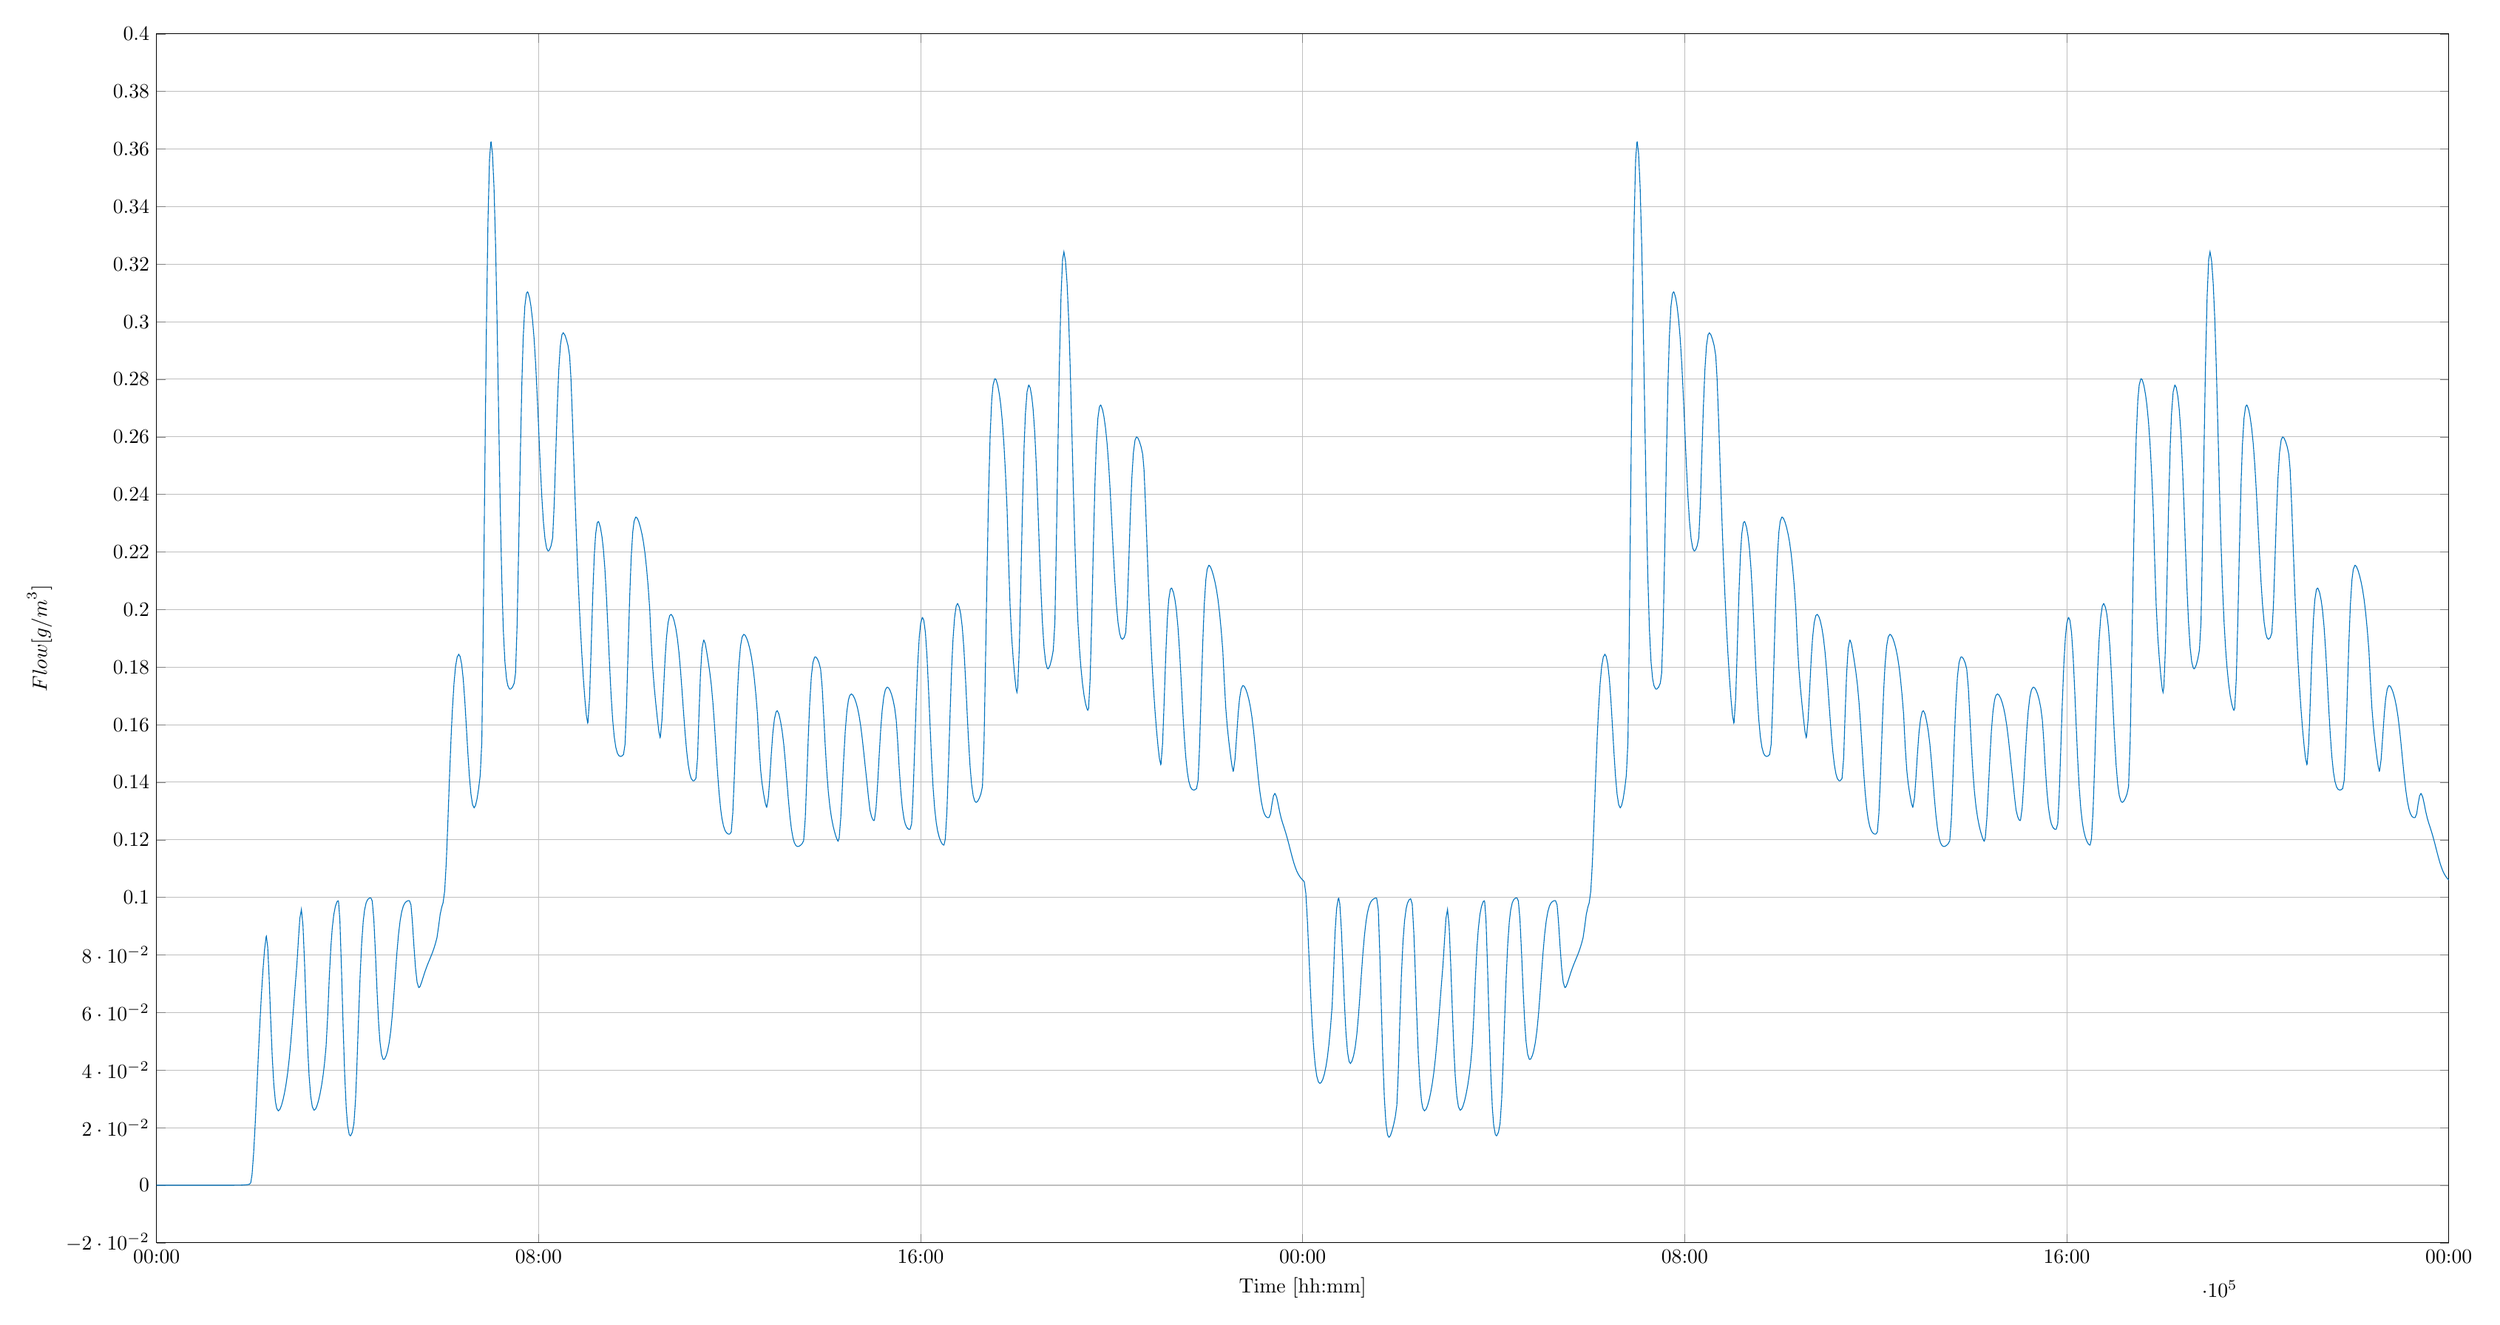
\begin{tikzpicture}

\begin{axis}[%
width=15.5in,
height=8.175in,
at={(2.6in,1.103in)},
scale only axis,
xmin=1,
xmax=172801,
xtick={1,28801,57601,86401,115201,144001,172801},
xticklabels={{00:00},{08:00},{16:00},{00:00},{08:00},{16:00},{00:00},{},{},{}},
xlabel={Time [hh:mm]},
xmajorgrids,
ymin=-0.02,
ymax=0.4,
ylabel={$\text{Flow [g/m}^\text{3}\text{]}$},
ymajorgrids,
axis background/.style={fill=white}
]
\addplot [color=mycolor1,solid,forget plot]
  table[row sep=crcr]{%
1	0\\
121	2.76444442474818e-109\\
241	3.26073009656065e-101\\
361	1.48722057706843e-94\\
481	9.07390854028621e-89\\
601	1.30076980586151e-83\\
701	1.08231091808059e-79\\
821	2.34738673163703e-75\\
941	1.3221333746199e-71\\
1061	3.20198537091244e-68\\
1181	5.82305692307098e-65\\
1281	2.4454529018171e-62\\
1401	2.56257479015984e-59\\
1521	1.86758071874072e-56\\
1641	9.43803249298235e-54\\
1761	3.39269645825311e-51\\
1861	3.59818145508685e-49\\
1981	7.43145424886407e-47\\
2101	1.16307577120233e-44\\
2221	1.36721652521903e-42\\
2341	1.68660368903054e-40\\
2441	2.35170957410801e-38\\
2561	1.30216127876707e-35\\
2681	5.85644996006396e-33\\
2801	2.24306122131333e-30\\
2921	7.60106686999932e-28\\
3021	9.43709554482937e-26\\
3141	5.90013951008352e-24\\
3261	1.46846532824227e-22\\
3381	2.2857813314748e-21\\
3501	1.97863169905587e-20\\
3601	7.73043630786215e-20\\
3721	2.56726045688387e-19\\
3841	6.26014920021868e-19\\
3961	1.31614841955074e-18\\
4081	2.72131669579753e-18\\
4201	6.30987738515826e-18\\
4301	1.51616521416971e-17\\
4421	5.60851788410215e-17\\
4541	2.6339333933766e-16\\
4661	1.44015306390873e-15\\
4781	8.3680115338951e-15\\
4881	3.58922621658711e-14\\
5001	1.95645240511166e-13\\
5121	9.94480128372167e-13\\
5241	4.70720404733287e-12\\
5361	2.09076018752307e-11\\
5461	7.41644489455555e-11\\
5581	7.24214793184579e-10\\
5701	3.19707992924011e-08\\
5821	5.70608545570831e-07\\
5941	1.80415957151033e-06\\
6041	3.81554329006679e-06\\
6161	8.96025772167814e-06\\
6281	2.05370658114337e-05\\
6401	4.18604942471306e-05\\
6521	7.2710127704623e-05\\
6621	0.000104304049087269\\
6741	0.000148111320476602\\
6861	0.000200586684032383\\
6981	0.000293352401992236\\
7101	0.000803797805528758\\
7201	0.00373316427553855\\
7321	0.0112988676031603\\
7441	0.0216265958635804\\
7561	0.0335097595848744\\
7681	0.0456943510219533\\
7801	0.0571866413478213\\
7901	0.0657777879623588\\
8021	0.0746358522261538\\
8141	0.0817601962521725\\
8261	0.0863572379239651\\
8281	0.0865351944787299\\
8381	0.0826868352217583\\
8481	0.0729328729720781\\
8601	0.0581850217639591\\
8721	0.044725357603887\\
8841	0.0349653661350658\\
8961	0.0291117635460206\\
9061	0.0266879469917678\\
9181	0.0258176888199261\\
9301	0.0263465314669768\\
9421	0.0277559180191354\\
9541	0.0297924228569586\\
9641	0.0319095831763245\\
9761	0.0350096550170574\\
9881	0.0388979610481673\\
10001	0.0437850540515898\\
10121	0.0497235509226516\\
10221	0.0553393938893703\\
10341	0.0625459979732243\\
10461	0.0698120774104384\\
10581	0.0767734203868196\\
10701	0.0856814291484519\\
10801	0.0926672708924115\\
10921	0.0958384827779321\\
11041	0.0900904191980293\\
11161	0.0769023939612189\\
11281	0.0611460041273074\\
11401	0.0469646731364804\\
11501	0.0380020148584435\\
11621	0.0309441692446212\\
11741	0.0273062648604276\\
11861	0.0261019009205255\\
11881	0.0260683183108994\\
11981	0.0264142750430167\\
12081	0.0274151105189277\\
12201	0.0292408712994812\\
12321	0.0316333360010084\\
12441	0.0346201085339089\\
12561	0.0383691355726851\\
12661	0.0422572667088365\\
12781	0.0482707642453505\\
12901	0.0586878405116733\\
13021	0.0720749340657065\\
13141	0.0827154885680492\\
13241	0.0890266252514835\\
13361	0.0939938169869922\\
13481	0.0968879064001237\\
13601	0.0984353528010755\\
13681	0.098813076786567\\
13721	0.0985348075014154\\
13821	0.0920427152472036\\
13941	0.075298872422749\\
14061	0.0558640981645994\\
14181	0.0387744884664413\\
14301	0.0267587617468617\\
14401	0.0208505283618553\\
14521	0.0176859050948064\\
14601	0.0171756347194794\\
14641	0.0172450864809872\\
14761	0.0184330083529576\\
14881	0.021446006624673\\
15001	0.0296915590538805\\
15101	0.0411250864689163\\
15221	0.0570253559853099\\
15341	0.0720784400230032\\
15461	0.0838664180283296\\
15581	0.0916844984904187\\
15681	0.0955974324496832\\
15801	0.0981331548392821\\
15921	0.0992804902052318\\
16041	0.0997381701301001\\
16121	0.0998281957990698\\
16161	0.0997895878738131\\
16261	0.0987248170524495\\
16381	0.0922400150811175\\
16501	0.0807971195713268\\
16621	0.0676300350816622\\
16741	0.0563839869388142\\
16841	0.0498732752106481\\
16961	0.0454520402678986\\
17081	0.043803653695271\\
17121	0.0436862670521838\\
17201	0.0439124307957137\\
17321	0.0451172938670885\\
17421	0.0467706947342416\\
17541	0.0496130963654136\\
17661	0.0537529616926854\\
17781	0.0595329505449419\\
17901	0.0667566967582858\\
18001	0.0732942416336339\\
18121	0.0808092376522041\\
18241	0.0871209626258829\\
18361	0.0918274376970769\\
18481	0.0949946886522725\\
18601	0.096941432295222\\
18701	0.0979007717822553\\
18821	0.0985342103493651\\
18941	0.0988213011868767\\
19021	0.0988838206502504\\
19061	0.0988634962711278\\
19181	0.0973930870815826\\
19281	0.091820003039776\\
19401	0.0832884205445895\\
19521	0.0755208977191211\\
19641	0.0705093124587236\\
19761	0.0686969434456523\\
19781	0.0686581463141937\\
19861	0.069028636703792\\
19981	0.0704887651006929\\
20101	0.0722625828888848\\
20221	0.0739834574284226\\
20341	0.0755580487674279\\
20441	0.0767629098487123\\
20561	0.078119337603574\\
20681	0.0794456720437077\\
20801	0.0808419954283449\\
20921	0.0824217880713266\\
21021	0.0839297245223279\\
21141	0.0860207744781929\\
21261	0.0898616104111471\\
21381	0.094105463313591\\
21501	0.0966445624733291\\
21601	0.0981197156835501\\
21721	0.102235546964558\\
21841	0.112129540365941\\
21961	0.12605362214973\\
22081	0.141321077674951\\
22201	0.15530552000296\\
22301	0.165061165884014\\
22421	0.174179084932181\\
22541	0.180230638075287\\
22661	0.183465745680596\\
22781	0.184434296028901\\
22881	0.183739374849786\\
23001	0.181005509135909\\
23121	0.17581923070715\\
23241	0.168138344869129\\
23361	0.158781849473533\\
23461	0.150759823566521\\
23581	0.142208756037235\\
23701	0.135881187917368\\
23821	0.132230364372004\\
23941	0.131130031839158\\
24041	0.131846886458409\\
24161	0.134221342645957\\
24281	0.13782272928218\\
24401	0.142486652793004\\
24521	0.154054375188698\\
24621	0.190959276274271\\
24741	0.245205232480758\\
24861	0.295861511812221\\
24981	0.333959414916128\\
25101	0.356370928796083\\
25201	0.362400038612471\\
25221	0.362449227844972\\
25321	0.358558336352734\\
25441	0.34656215833316\\
25561	0.326286055306966\\
25681	0.297589785657611\\
25801	0.264344023267989\\
25901	0.237636310542211\\
26021	0.211249512533777\\
26141	0.192934030413059\\
26261	0.181874908234323\\
26381	0.17598251860991\\
26481	0.173569857472627\\
26601	0.172443804646804\\
26661	0.172340339924044\\
26721	0.172446936843953\\
26841	0.173122047083024\\
26961	0.174423946408175\\
27061	0.177881861677216\\
27181	0.19457685767797\\
27301	0.222179251344584\\
27421	0.252857116716482\\
27541	0.279006975955229\\
27641	0.294398262045764\\
27761	0.305257376056342\\
27881	0.309743313529039\\
27961	0.310363764805266\\
28001	0.310189595932031\\
28121	0.308298112651378\\
28221	0.30550560875377\\
28341	0.30077740943752\\
28461	0.294149472214426\\
28581	0.285103013157337\\
28701	0.273760271999224\\
28801	0.26325111097251\\
28921	0.250641721541545\\
29041	0.239415061043866\\
29161	0.230613195677043\\
29281	0.224655350174716\\
29401	0.221401036313713\\
29501	0.220402566991141\\
29541	0.220352308570717\\
29621	0.220722928794362\\
29741	0.222164715112768\\
29861	0.224910230644686\\
29981	0.237004287914564\\
30081	0.25197894954146\\
30201	0.26947746203323\\
30321	0.283212177400575\\
30441	0.291688241189471\\
30561	0.295461523588751\\
30661	0.296144165483163\\
30781	0.295390894574562\\
30901	0.293799003293314\\
31021	0.29166144491173\\
31141	0.288114941178216\\
31241	0.28025659262562\\
31361	0.265232903817847\\
31481	0.248328749647045\\
31601	0.231881487962185\\
31721	0.217077755073808\\
31821	0.206165766758145\\
31941	0.194601332299876\\
32061	0.184483894414564\\
32181	0.175704716664847\\
32301	0.168268279604855\\
32401	0.163257741033995\\
32501	0.160533155403223\\
32521	0.160704787694308\\
32641	0.169069938537596\\
32761	0.186165535156872\\
32881	0.204707098149095\\
33001	0.218959384889719\\
33101	0.226206176709738\\
33221	0.230089532906655\\
33301	0.230574170469499\\
33341	0.230381426026662\\
33461	0.22857152104133\\
33581	0.225247979250713\\
33681	0.221158147397813\\
33801	0.213993289040051\\
33921	0.204018884006892\\
34041	0.192068348437596\\
34161	0.179843946989063\\
34261	0.170700116555285\\
34381	0.161945051628519\\
34501	0.155872957783439\\
34621	0.152133897013863\\
34741	0.150104683300799\\
34841	0.149287601280144\\
34961	0.148967437341586\\
34981	0.148963556713094\\
35081	0.149100170834221\\
35201	0.149635402067089\\
35321	0.153257198710477\\
35421	0.165240606342631\\
35541	0.184399688743802\\
35661	0.203419869189687\\
35781	0.218076972798879\\
35901	0.227016064682697\\
36001	0.23069821443112\\
36121	0.232113467287479\\
36141	0.23214226040682\\
36241	0.231728685638816\\
36361	0.230408998964677\\
36481	0.228504339055521\\
36601	0.226072298733475\\
36701	0.223524720845147\\
36821	0.219550171804097\\
36941	0.21432880171776\\
37061	0.207964365497901\\
37181	0.199938116335806\\
37281	0.18966011722188\\
37401	0.17987765400728\\
37521	0.172900466814579\\
37641	0.167146540269181\\
37761	0.161868058659228\\
37861	0.15778374822096\\
37961	0.155524599992351\\
37981	0.155722022791258\\
38101	0.161563826339077\\
38221	0.172361400511875\\
38341	0.183266025455923\\
38441	0.190210219111162\\
38561	0.195435705297605\\
38681	0.197845003232295\\
38781	0.19831702272898\\
38801	0.198287833444919\\
38921	0.197456733799869\\
39021	0.196053409276952\\
39141	0.193578211653186\\
39261	0.190061767603159\\
39381	0.185174650340202\\
39501	0.178803690219295\\
39601	0.172613496742503\\
39721	0.164761931019481\\
39841	0.157273333373539\\
39961	0.150901346639528\\
40081	0.14608399179095\\
40201	0.142896890010242\\
40301	0.141349413330753\\
40421	0.140545815515901\\
40481	0.140476830392724\\
40541	0.140581677343265\\
40661	0.141357193242881\\
40781	0.14829499045621\\
40881	0.16215463176129\\
41001	0.177310697625528\\
41121	0.18643618865635\\
41241	0.189352929679984\\
41261	0.189381692068831\\
41361	0.188218927961049\\
41461	0.185687662657421\\
41581	0.182131489605975\\
41701	0.17840351946569\\
41821	0.173829269058885\\
41941	0.167662560249501\\
42041	0.161269787077822\\
42161	0.152674067949021\\
42281	0.144103925471601\\
42401	0.136629195329265\\
42521	0.130878232015858\\
42621	0.127465531162475\\
42741	0.124770652300076\\
42861	0.123199225306756\\
42981	0.122368684239336\\
43101	0.122011523462945\\
43161	0.121961669276891\\
43201	0.121976114909382\\
43321	0.122657046477994\\
43441	0.129250858057506\\
43561	0.142599632895036\\
43681	0.158152267805625\\
43801	0.172038684923018\\
43901	0.180673107591385\\
44021	0.187247540583869\\
44141	0.190429779191366\\
44261	0.191362910256903\\
44281	0.19137338978929\\
44381	0.191000071862703\\
44481	0.190096520450621\\
44601	0.18850243241025\\
44721	0.186399706585078\\
44841	0.183665747644786\\
44961	0.180030708272319\\
45061	0.176147443129934\\
45181	0.170509595273739\\
45301	0.163671875801723\\
45421	0.152557206176753\\
45541	0.144167057173425\\
45641	0.13977353708981\\
45761	0.136000964153427\\
45881	0.13293299401527\\
45981	0.131312697952015\\
46001	0.131313884289518\\
46121	0.134553626264236\\
46221	0.14075560796039\\
46341	0.149660221944227\\
46461	0.157200937507326\\
46581	0.162037529999454\\
46701	0.164400201352814\\
46781	0.164853174913647\\
46801	0.164832944137965\\
46921	0.163632767214168\\
47041	0.161107698352983\\
47161	0.157785010982712\\
47281	0.153281217945739\\
47401	0.147262143674965\\
47501	0.141474810042095\\
47621	0.134499314805761\\
47741	0.128401024389963\\
47861	0.12373798716792\\
47981	0.120599340442698\\
48081	0.118991743735239\\
48201	0.117979589203081\\
48321	0.117658930644392\\
48341	0.11765348402296\\
48441	0.117774121913079\\
48561	0.118154729039946\\
48661	0.118612798373225\\
48781	0.119682334701675\\
48901	0.127232587120486\\
49021	0.141559719128736\\
49141	0.156819004579974\\
49241	0.167622204077935\\
49361	0.176688597899813\\
49481	0.181565089507746\\
49601	0.18337135604781\\
49661	0.183556136628811\\
49721	0.183439751592704\\
49821	0.182793720121873\\
49941	0.181489621315064\\
50061	0.179292468636039\\
50181	0.172893329321038\\
50301	0.162412387719161\\
50401	0.153420083023936\\
50521	0.143985214617625\\
50641	0.136721234384497\\
50761	0.131464654692538\\
50881	0.127676879895888\\
51001	0.124842200464449\\
51101	0.122949382333449\\
51221	0.121075702955252\\
51341	0.119702805070356\\
51381	0.11952788265263\\
51461	0.120716992363927\\
51581	0.12766532233538\\
51681	0.136583895433063\\
51801	0.148144476204113\\
51921	0.157925317147659\\
52041	0.164700558713691\\
52161	0.168620683096674\\
52261	0.170180595157329\\
52381	0.170677176967025\\
52501	0.170226748345767\\
52621	0.16915012086271\\
52741	0.167568895953961\\
52841	0.165844326380381\\
52961	0.163147803253587\\
53081	0.159590621531531\\
53201	0.155148956105837\\
53321	0.150059524207688\\
53421	0.145636829658566\\
53541	0.140525708619248\\
53661	0.135029925699036\\
53781	0.13032095290372\\
53901	0.128026993107315\\
54001	0.126986151207112\\
54081	0.126662727796166\\
54121	0.126949573163973\\
54241	0.131171911948409\\
54361	0.139597528008769\\
54481	0.149795028367627\\
54601	0.159042032643331\\
54701	0.164928062108658\\
54821	0.169635112726718\\
54941	0.172127887208575\\
55061	0.172994115278823\\
55101	0.173023610835978\\
55181	0.172790026536906\\
55281	0.172054811642347\\
55401	0.170636194296596\\
55521	0.168636785371471\\
55641	0.165873358462534\\
55761	0.161591393280517\\
55861	0.154945457589166\\
55981	0.14528255795534\\
56101	0.137117979905838\\
56221	0.131223505102841\\
56341	0.127439560179417\\
56441	0.12553152169543\\
56561	0.124267082250608\\
56681	0.123715381526299\\
56761	0.123612153463821\\
56801	0.123649345169826\\
56921	0.125574459273521\\
57021	0.134461836301597\\
57141	0.15022856108207\\
57261	0.167033622737534\\
57381	0.181065067033485\\
57501	0.190613078033584\\
57601	0.195155006318666\\
57721	0.197200255159215\\
57741	0.197240146127899\\
57841	0.196239725498673\\
57961	0.191985517397728\\
58081	0.183687324804279\\
58201	0.171913928877112\\
58301	0.160885308412012\\
58421	0.148307152524947\\
58541	0.138079892240592\\
58661	0.130732791778715\\
58781	0.125849879755743\\
58881	0.123126198303436\\
59001	0.120906232011767\\
59121	0.119428194568761\\
59241	0.118472256767598\\
59341	0.118145380870026\\
59361	0.118190074738609\\
59461	0.120267865608977\\
59581	0.129783707782681\\
59701	0.145741871360121\\
59821	0.163999528989139\\
59941	0.179887700365845\\
60041	0.189638893070811\\
60161	0.197272343169687\\
60281	0.201223853463956\\
60381	0.202082963570214\\
60401	0.202039719446735\\
60521	0.200721354271436\\
60621	0.198432226273931\\
60741	0.193851937215477\\
60861	0.186478498199085\\
60981	0.176311060647995\\
61101	0.164697848259418\\
61201	0.155360387373203\\
61321	0.145994118447559\\
61441	0.139343182325883\\
61561	0.135336720101241\\
61681	0.133436605596514\\
61781	0.133003197212716\\
61801	0.133010264827357\\
61901	0.13339847186403\\
62021	0.13443645130343\\
62141	0.135912797440694\\
62261	0.138541222366259\\
62381	0.154339722301692\\
62481	0.178836242950003\\
62601	0.211292720107396\\
62721	0.240005968844867\\
62841	0.260660206831289\\
62961	0.272912733404425\\
63061	0.277996008262035\\
63181	0.280119732071379\\
63221	0.280197237720685\\
63301	0.279703599901562\\
63421	0.277749967471372\\
63541	0.274632147679877\\
63641	0.27109531883942\\
63761	0.265318162934674\\
63881	0.257326314366701\\
64001	0.247066816102083\\
64121	0.234443590519152\\
64221	0.218358203366507\\
64341	0.201566790257848\\
64461	0.190609938195688\\
64581	0.182769586273719\\
64701	0.176424504069943\\
64801	0.172306467614986\\
64861	0.171263122893414\\
64921	0.173035427820021\\
65041	0.186946229213372\\
65161	0.210829530589508\\
65281	0.236421128156293\\
65401	0.256813380523448\\
65501	0.268125687282547\\
65621	0.275590723263818\\
65741	0.277930383980442\\
65761	0.277960631332574\\
65861	0.277024225430913\\
65981	0.273891658491943\\
66081	0.269551276036794\\
66201	0.26162495989936\\
66321	0.250129236285442\\
66441	0.235628215262029\\
66561	0.21997817113277\\
66661	0.207714470863248\\
66781	0.195514421608528\\
66901	0.186885687300478\\
67021	0.181798176490625\\
67141	0.179639001401567\\
67201	0.179408208085315\\
67241	0.179502658873\\
67361	0.180706719462022\\
67481	0.18289101841963\\
67601	0.185894393680798\\
67721	0.195558479239143\\
67821	0.219845153721307\\
67941	0.25390420941741\\
68061	0.285375304487389\\
68181	0.308644284808578\\
68301	0.321600782112079\\
68401	0.324286784963207\\
68521	0.321051545410977\\
68641	0.313292233347647\\
68761	0.300851856036316\\
68881	0.283241929380423\\
69001	0.262080430134431\\
69101	0.243960805487934\\
69221	0.224160279141284\\
69341	0.207946562439016\\
69461	0.195450672786006\\
69581	0.186020109400799\\
69681	0.179952105098963\\
69801	0.174316337912046\\
69921	0.170122782750927\\
70041	0.167128065066903\\
70161	0.165258695409898\\
70201	0.165016240546719\\
70261	0.165650846176839\\
70381	0.176100298851315\\
70501	0.197066600792576\\
70621	0.221926515317262\\
70741	0.243822359421681\\
70841	0.256981609930431\\
70961	0.26643264370025\\
71081	0.270432425495679\\
71161	0.271032034634726\\
71201	0.270905932464713\\
71321	0.269327819821758\\
71421	0.266964706643336\\
71541	0.262987805622455\\
71661	0.257472198389372\\
71781	0.249943849565598\\
71901	0.240370569177064\\
72001	0.231323293537346\\
72121	0.220195683975667\\
72241	0.209954075442248\\
72361	0.201564800924851\\
72481	0.195500092227108\\
72601	0.191751868977007\\
72701	0.190159930843298\\
72801	0.189663880093336\\
72821	0.189670361301948\\
72941	0.190275598812515\\
73061	0.191950729823269\\
73181	0.201341548106624\\
73281	0.215069675033658\\
73401	0.231867273588921\\
73521	0.245605371446192\\
73641	0.254492699442806\\
73761	0.258811156387285\\
73861	0.259912966033707\\
73881	0.259951612719252\\
73981	0.25956622786065\\
74101	0.258306417073047\\
74221	0.256520726262827\\
74341	0.253914467017446\\
74441	0.24857133767195\\
74561	0.235597103045261\\
74681	0.220400372217847\\
74801	0.205624000178742\\
74921	0.192574315612604\\
75021	0.183209304417277\\
75141	0.173551875557043\\
75261	0.165298324230937\\
75381	0.158234061060133\\
75501	0.15228306816584\\
75601	0.148274354365806\\
75701	0.146117355505312\\
75721	0.146274342203287\\
75841	0.153488780250664\\
75961	0.168252448561592\\
76081	0.184389354393368\\
76201	0.196919437534008\\
76301	0.203374606123165\\
76421	0.206934892116526\\
76501	0.207463906400045\\
76541	0.207344393272843\\
76661	0.205903924359296\\
76781	0.203163489345831\\
76881	0.199784113846969\\
77001	0.193856669951267\\
77121	0.185517384546372\\
77241	0.17537705119807\\
77361	0.164845896829854\\
77461	0.156857778302487\\
77581	0.149104488963247\\
77701	0.143650756305557\\
77821	0.14024859131808\\
77941	0.138377980396506\\
78041	0.137611406345773\\
78161	0.137293376050632\\
78181	0.137285411031243\\
78281	0.137386294090374\\
78401	0.137828365466121\\
78521	0.140812628801669\\
78621	0.151683575344046\\
78741	0.169543445677966\\
78861	0.187562689120253\\
78981	0.201670924948195\\
79101	0.210391891731191\\
79201	0.213998003464363\\
79321	0.215344765943397\\
79341	0.215362782406269\\
79441	0.214902506977894\\
79561	0.213555779153269\\
79681	0.211674038239239\\
79801	0.20933923834926\\
79901	0.206958218931337\\
80021	0.203319786575603\\
80141	0.198560272953762\\
80261	0.192700269209154\\
80381	0.185606843368724\\
80481	0.176051742042344\\
80601	0.165972530152896\\
80721	0.159122369734596\\
80841	0.153898093117738\\
80961	0.149383802872718\\
81061	0.145968209769426\\
81161	0.143838306485295\\
81181	0.143909600234445\\
81301	0.148009069393978\\
81421	0.15600855728772\\
81541	0.164051419679521\\
81641	0.168998531229004\\
81761	0.17239869969676\\
81881	0.173566613990258\\
81901	0.173601790696433\\
82001	0.173305994888905\\
82121	0.172219858820626\\
82221	0.170887229276094\\
82341	0.168813215454325\\
82461	0.16608663008967\\
82581	0.162459730462448\\
82701	0.157818683855372\\
82801	0.153322074528439\\
82921	0.147581597054398\\
83041	0.142020124013407\\
83161	0.137163455853173\\
83281	0.13333961119089\\
83401	0.130634005210768\\
83501	0.129157890792863\\
83621	0.128139328191677\\
83741	0.127723426242987\\
83801	0.127679537507414\\
83861	0.127735528145708\\
83981	0.129073920658983\\
84081	0.13228060884382\\
84201	0.13528013083949\\
84301	0.13610471471387\\
84321	0.13607596826055\\
84441	0.134779341972954\\
84561	0.132209603864909\\
84661	0.129845760219501\\
84781	0.127485728158148\\
84901	0.125634681000579\\
85021	0.123938669996316\\
85141	0.122154457359979\\
85241	0.120540554356715\\
85361	0.118462246897481\\
85481	0.116300692518993\\
85601	0.114173519195394\\
85721	0.112205682124206\\
85821	0.110757565491432\\
85941	0.109292774528014\\
86061	0.108126145352853\\
86181	0.107222956155136\\
86301	0.106530895557899\\
86401	0.10606781508754\\
86521	0.105396385542433\\
86641	0.101352444703132\\
86761	0.0915214974179343\\
86881	0.079013924901606\\
87001	0.0663954500967941\\
87101	0.0571574755590284\\
87221	0.0482270355502681\\
87341	0.0418474964728464\\
87461	0.0379312981931191\\
87581	0.0359613280772862\\
87681	0.0354084324459614\\
87701	0.0353925413533537\\
87801	0.0357072494607494\\
87921	0.0368298549836208\\
88041	0.0386844215744185\\
88161	0.0413382375103552\\
88261	0.0443089741033974\\
88381	0.0489852632642238\\
88501	0.0549408599599261\\
88621	0.0621805240913447\\
88741	0.0752630619824175\\
88841	0.0877733582843575\\
88961	0.0961973930661932\\
89081	0.0995362661481415\\
89121	0.0997104605364454\\
89201	0.0977193372512125\\
89321	0.088587691191014\\
89421	0.0776581082844324\\
89541	0.0640276298897265\\
89661	0.0531355694411123\\
89781	0.046296595532506\\
89901	0.0429876836994137\\
90001	0.0422884537028883\\
90121	0.0431251941842938\\
90241	0.0450162827679448\\
90361	0.0479212086862721\\
90481	0.0523336733945131\\
90601	0.0585590402551135\\
90701	0.0648561869341357\\
90821	0.0729241147950218\\
90941	0.0805426706333973\\
91061	0.0869236622005121\\
91181	0.091740756517892\\
91281	0.0946041755209932\\
91401	0.0969046832309118\\
91521	0.0982947902188968\\
91641	0.099087557460094\\
91761	0.099518107885319\\
91861	0.0997104855603433\\
91921	0.0997623623439941\\
91981	0.0996924774934149\\
92101	0.0958032592869401\\
92221	0.0799504720793797\\
92341	0.0600779459060714\\
92441	0.0444580723153603\\
92561	0.0300526548277492\\
92681	0.0213473195257541\\
92801	0.0174757970533029\\
92901	0.0166663661560637\\
92921	0.0166769738231671\\
93021	0.0173090120672348\\
93141	0.0189241943011555\\
93261	0.0211003789718111\\
93381	0.0237290078885917\\
93501	0.0278231141810732\\
93601	0.0383545077997871\\
93721	0.0565417565924759\\
93841	0.0726578301485952\\
93961	0.0844401753137214\\
94081	0.0918929424667913\\
94201	0.0960939580249704\\
94301	0.0979876416762785\\
94421	0.0991419521330638\\
94541	0.0995449099913866\\
94661	0.097654395688874\\
94781	0.0876884952362526\\
94881	0.0752907026877627\\
95001	0.059085914220699\\
95121	0.0450497285221234\\
95241	0.0350760579449971\\
95361	0.0291481765836666\\
95461	0.0267025625404729\\
95581	0.0258229929649201\\
95701	0.0263487165384103\\
95821	0.0277569516852642\\
95941	0.0297929825634608\\
96041	0.0319099518528783\\
96161	0.0350099005735165\\
96281	0.0388981383783582\\
96401	0.0437851900719673\\
96521	0.0497236600577751\\
96621	0.0553394869799584\\
96741	0.0625460762042433\\
96861	0.0698121434639444\\
96981	0.0767734754071093\\
97101	0.0856814678333269\\
97201	0.0926672940409395\\
97321	0.0958384937552925\\
97441	0.0900904225004552\\
97561	0.0769023947988\\
97681	0.061146004322035\\
97801	0.0469646731785606\\
97901	0.0380020148696363\\
98021	0.0309441692468055\\
98141	0.0273062648608521\\
98261	0.0261019009206145\\
98281	0.0260683183109688\\
98381	0.0264142750430377\\
98481	0.0274151105189347\\
98601	0.0292408712994832\\
98721	0.0316333360010091\\
98841	0.0346201085339091\\
98961	0.0383691355726852\\
99061	0.0422572667088366\\
99181	0.0482707642453505\\
99301	0.0586878405116733\\
99421	0.0720749340657065\\
99541	0.0827154885680492\\
99641	0.0890266252514835\\
99761	0.0939938169869922\\
99881	0.0968879064001237\\
100001	0.0984353528010755\\
100081	0.0988130767865669\\
100121	0.0985348075014154\\
100221	0.0920427152472036\\
100341	0.075298872422749\\
100461	0.0558640981645994\\
100581	0.0387744884664413\\
100701	0.0267587617468617\\
100801	0.0208505283618553\\
100921	0.0176859050948064\\
101001	0.0171756347194794\\
101041	0.0172450864809872\\
101161	0.0184330083529576\\
101281	0.021446006624673\\
101401	0.0296915590538805\\
101501	0.0411250864689163\\
101621	0.0570253559853099\\
101741	0.0720784400230032\\
101861	0.0838664180283296\\
101981	0.0916844984904187\\
102081	0.0955974324496832\\
102201	0.0981331548392821\\
102321	0.0992804902052318\\
102441	0.0997381701301001\\
102521	0.0998281957990698\\
102561	0.0997895878738131\\
102661	0.0987248170524495\\
102781	0.0922400150811175\\
102901	0.0807971195713268\\
103021	0.0676300350816622\\
103141	0.0563839869388142\\
103241	0.0498732752106481\\
103361	0.0454520402678986\\
103481	0.043803653695271\\
103521	0.0436862670521838\\
103601	0.0439124307957137\\
103721	0.0451172938670885\\
103821	0.0467706947342416\\
103941	0.0496130963654136\\
104061	0.0537529616926854\\
104181	0.0595329505449419\\
104301	0.0667566967582858\\
104401	0.0732942416336339\\
104521	0.0808092376522041\\
104641	0.0871209626258829\\
104761	0.0918274376970769\\
104881	0.0949946886522725\\
105001	0.096941432295222\\
105101	0.0979007717822553\\
105221	0.0985342103493651\\
105341	0.0988213011868767\\
105421	0.0988838206502504\\
105461	0.0988634962711278\\
105581	0.0973930870815826\\
105681	0.091820003039776\\
105801	0.0832884205445895\\
105921	0.0755208977191211\\
106041	0.0705093124587236\\
106161	0.0686969434456523\\
106181	0.0686581463141937\\
106261	0.069028636703792\\
106381	0.0704887651006929\\
106501	0.0722625828888848\\
106621	0.0739834574284226\\
106741	0.0755580487674279\\
106841	0.0767629098487123\\
106961	0.078119337603574\\
107081	0.0794456720437077\\
107201	0.0808419954283449\\
107321	0.0824217880713266\\
107421	0.0839297245223279\\
107541	0.0860207744781929\\
107661	0.0898616104111471\\
107781	0.094105463313591\\
107901	0.0966445624733291\\
108001	0.0981197156835501\\
108121	0.102235546964558\\
108241	0.112129540365941\\
108361	0.12605362214973\\
108481	0.141321077674951\\
108601	0.15530552000296\\
108701	0.165061165884014\\
108821	0.174179084932181\\
108941	0.180230638075287\\
109061	0.183465745680596\\
109181	0.184434296028901\\
109281	0.183739374849786\\
109401	0.181005509135909\\
109521	0.17581923070715\\
109641	0.168138344869129\\
109761	0.158781849473533\\
109861	0.150759823566521\\
109981	0.142208756037235\\
110101	0.135881187917368\\
110221	0.132230364372004\\
110341	0.131130031839158\\
110441	0.131846886458409\\
110561	0.134221342645957\\
110681	0.13782272928218\\
110801	0.142486652793004\\
110921	0.154054375188698\\
111021	0.190959276274271\\
111141	0.245205232480758\\
111261	0.295861511812221\\
111381	0.333959414916128\\
111501	0.356370928796083\\
111601	0.362400038612471\\
111621	0.362449227844972\\
111721	0.358558336352734\\
111841	0.34656215833316\\
111961	0.326286055306966\\
112081	0.297589785657611\\
112201	0.264344023267989\\
112301	0.237636310542211\\
112421	0.211249512533777\\
112541	0.192934030413059\\
112661	0.181874908234323\\
112781	0.17598251860991\\
112881	0.173569857472627\\
113001	0.172443804646804\\
113061	0.172340339924044\\
113121	0.172446936843953\\
113241	0.173122047083024\\
113361	0.174423946408175\\
113461	0.177881861677216\\
113581	0.19457685767797\\
113701	0.222179251344584\\
113821	0.252857116716482\\
113941	0.279006975955229\\
114041	0.294398262045764\\
114161	0.305257376056342\\
114281	0.309743313529039\\
114361	0.310363764805266\\
114401	0.310189595932031\\
114521	0.308298112651378\\
114621	0.30550560875377\\
114741	0.30077740943752\\
114861	0.294149472214426\\
114981	0.285103013157337\\
115101	0.273760271999224\\
115201	0.26325111097251\\
115321	0.250641721541545\\
115441	0.239415061043866\\
115561	0.230613195677043\\
115681	0.224655350174716\\
115801	0.221401036313713\\
115901	0.220402566991141\\
115941	0.220352308570717\\
116021	0.220722928794362\\
116141	0.222164715112768\\
116261	0.224910230644686\\
116381	0.237004287914564\\
116481	0.25197894954146\\
116601	0.26947746203323\\
116721	0.283212177400575\\
116841	0.291688241189471\\
116961	0.295461523588751\\
117061	0.296144165483163\\
117181	0.295390894574562\\
117301	0.293799003293314\\
117421	0.29166144491173\\
117541	0.288114941178216\\
117641	0.28025659262562\\
117761	0.265232903817847\\
117881	0.248328749647045\\
118001	0.231881487962185\\
118121	0.217077755073808\\
118221	0.206165766758145\\
118341	0.194601332299876\\
118461	0.184483894414564\\
118581	0.175704716664847\\
118701	0.168268279604855\\
118801	0.163257741033995\\
118901	0.160533155403223\\
118921	0.160704787694308\\
119041	0.169069938537596\\
119161	0.186165535156872\\
119281	0.204707098149095\\
119401	0.218959384889719\\
119501	0.226206176709738\\
119621	0.230089532906655\\
119701	0.230574170469499\\
119741	0.230381426026662\\
119861	0.22857152104133\\
119981	0.225247979250713\\
120081	0.221158147397813\\
120201	0.213993289040051\\
120321	0.204018884006892\\
120441	0.192068348437596\\
120561	0.179843946989063\\
120661	0.170700116555285\\
120781	0.161945051628519\\
120901	0.155872957783439\\
121021	0.152133897013863\\
121141	0.150104683300799\\
121241	0.149287601280144\\
121361	0.148967437341586\\
121381	0.148963556713094\\
121481	0.149100170834221\\
121601	0.149635402067089\\
121721	0.153257198710477\\
121821	0.165240606342631\\
121941	0.184399688743802\\
122061	0.203419869189687\\
122181	0.218076972798879\\
122301	0.227016064682697\\
122401	0.23069821443112\\
122521	0.232113467287479\\
122541	0.23214226040682\\
122641	0.231728685638816\\
122761	0.230408998964677\\
122881	0.228504339055521\\
123001	0.226072298733475\\
123101	0.223524720845147\\
123221	0.219550171804097\\
123341	0.21432880171776\\
123461	0.207964365497901\\
123581	0.199938116335806\\
123681	0.18966011722188\\
123801	0.17987765400728\\
123921	0.172900466814579\\
124041	0.167146540269181\\
124161	0.161868058659228\\
124261	0.15778374822096\\
124361	0.155524599992351\\
124381	0.155722022791258\\
124501	0.161563826339077\\
124621	0.172361400511875\\
124741	0.183266025455923\\
124841	0.190210219111162\\
124961	0.195435705297605\\
125081	0.197845003232295\\
125181	0.19831702272898\\
125201	0.198287833444919\\
125321	0.197456733799869\\
125421	0.196053409276952\\
125541	0.193578211653186\\
125661	0.190061767603159\\
125781	0.185174650340202\\
125901	0.178803690219295\\
126001	0.172613496742503\\
126121	0.164761931019481\\
126241	0.157273333373539\\
126361	0.150901346639528\\
126481	0.14608399179095\\
126601	0.142896890010242\\
126701	0.141349413330753\\
126821	0.140545815515901\\
126881	0.140476830392724\\
126941	0.140581677343265\\
127061	0.141357193242881\\
127181	0.14829499045621\\
127281	0.16215463176129\\
127401	0.177310697625528\\
127521	0.18643618865635\\
127641	0.189352929679984\\
127661	0.189381692068831\\
127761	0.188218927961049\\
127861	0.185687662657421\\
127981	0.182131489605975\\
128101	0.17840351946569\\
128221	0.173829269058885\\
128341	0.167662560249501\\
128441	0.161269787077822\\
128561	0.152674067949021\\
128681	0.144103925471601\\
128801	0.136629195329265\\
128921	0.130878232015858\\
129021	0.127465531162475\\
129141	0.124770652300076\\
129261	0.123199225306756\\
129381	0.122368684239336\\
129501	0.122011523462945\\
129561	0.121961669276891\\
129601	0.121976114909382\\
129721	0.122657046477994\\
129841	0.129250858057506\\
129961	0.142599632895036\\
130081	0.158152267805625\\
130201	0.172038684923018\\
130301	0.180673107591385\\
130421	0.187247540583869\\
130541	0.190429779191366\\
130661	0.191362910256903\\
130681	0.19137338978929\\
130781	0.191000071862703\\
130881	0.190096520450621\\
131001	0.18850243241025\\
131121	0.186399706585078\\
131241	0.183665747644786\\
131361	0.180030708272319\\
131461	0.176147443129934\\
131581	0.170509595273739\\
131701	0.163671875801723\\
131821	0.152557206176753\\
131941	0.144167057173425\\
132041	0.13977353708981\\
132161	0.136000964153427\\
132281	0.13293299401527\\
132381	0.131312697952015\\
132401	0.131313884289518\\
132521	0.134553626264236\\
132621	0.14075560796039\\
132741	0.149660221944227\\
132861	0.157200937507326\\
132981	0.162037529999454\\
133101	0.164400201352814\\
133181	0.164853174913647\\
133201	0.164832944137965\\
133321	0.163632767214168\\
133441	0.161107698352983\\
133561	0.157785010982712\\
133681	0.153281217945739\\
133801	0.147262143674965\\
133901	0.141474810042095\\
134021	0.134499314805761\\
134141	0.128401024389963\\
134261	0.12373798716792\\
134381	0.120599340442698\\
134481	0.118991743735239\\
134601	0.117979589203081\\
134721	0.117658930644392\\
134741	0.11765348402296\\
134841	0.117774121913079\\
134961	0.118154729039946\\
135061	0.118612798373225\\
135181	0.119682334701675\\
135301	0.127232587120486\\
135421	0.141559719128736\\
135541	0.156819004579974\\
135641	0.167622204077935\\
135761	0.176688597899813\\
135881	0.181565089507746\\
136001	0.18337135604781\\
136061	0.183556136628811\\
136121	0.183439751592704\\
136221	0.182793720121873\\
136341	0.181489621315064\\
136461	0.179292468636039\\
136581	0.172893329321038\\
136701	0.162412387719161\\
136801	0.153420083023936\\
136921	0.143985214617625\\
137041	0.136721234384497\\
137161	0.131464654692538\\
137281	0.127676879895888\\
137401	0.124842200464449\\
137501	0.122949382333449\\
137621	0.121075702955252\\
137741	0.119702805070356\\
137781	0.11952788265263\\
137861	0.120716992363927\\
137981	0.12766532233538\\
138081	0.136583895433063\\
138201	0.148144476204113\\
138321	0.157925317147659\\
138441	0.164700558713691\\
138561	0.168620683096674\\
138661	0.170180595157329\\
138781	0.170677176967025\\
138901	0.170226748345767\\
139021	0.16915012086271\\
139141	0.167568895953961\\
139241	0.165844326380381\\
139361	0.163147803253587\\
139481	0.159590621531531\\
139601	0.155148956105837\\
139721	0.150059524207688\\
139821	0.145636829658566\\
139941	0.140525708619248\\
140061	0.135029925699036\\
140181	0.13032095290372\\
140301	0.128026993107315\\
140401	0.126986151207112\\
140481	0.126662727796166\\
140521	0.126949573163973\\
140641	0.131171911948409\\
140761	0.139597528008769\\
140881	0.149795028367627\\
141001	0.159042032643331\\
141101	0.164928062108658\\
141221	0.169635112726718\\
141341	0.172127887208575\\
141461	0.172994115278823\\
141501	0.173023610835978\\
141581	0.172790026536906\\
141681	0.172054811642347\\
141801	0.170636194296596\\
141921	0.168636785371471\\
142041	0.165873358462534\\
142161	0.161591393280517\\
142261	0.154945457589166\\
142381	0.14528255795534\\
142501	0.137117979905838\\
142621	0.131223505102841\\
142741	0.127439560179417\\
142841	0.12553152169543\\
142961	0.124267082250608\\
143081	0.123715381526299\\
143161	0.123612153463821\\
143201	0.123649345169826\\
143321	0.125574459273521\\
143421	0.134461836301597\\
143541	0.15022856108207\\
143661	0.167033622737534\\
143781	0.181065067033485\\
143901	0.190613078033584\\
144001	0.195155006318666\\
144121	0.197200255159215\\
144141	0.197240146127899\\
144241	0.196239725498673\\
144361	0.191985517397728\\
144481	0.183687324804279\\
144601	0.171913928877112\\
144701	0.160885308412012\\
144821	0.148307152524947\\
144941	0.138079892240592\\
145061	0.130732791778715\\
145181	0.125849879755743\\
145281	0.123126198303436\\
145401	0.120906232011767\\
145521	0.119428194568761\\
145641	0.118472256767598\\
145741	0.118145380870026\\
145761	0.118190074738609\\
145861	0.120267865608977\\
145981	0.129783707782681\\
146101	0.145741871360121\\
146221	0.163999528989139\\
146341	0.179887700365845\\
146441	0.189638893070811\\
146561	0.197272343169687\\
146681	0.201223853463956\\
146781	0.202082963570214\\
146801	0.202039719446735\\
146921	0.200721354271436\\
147021	0.198432226273931\\
147141	0.193851937215477\\
147261	0.186478498199085\\
147381	0.176311060647995\\
147501	0.164697848259418\\
147601	0.155360387373203\\
147721	0.145994118447559\\
147841	0.139343182325883\\
147961	0.135336720101241\\
148081	0.133436605596514\\
148181	0.133003197212716\\
148201	0.133010264827357\\
148301	0.13339847186403\\
148421	0.13443645130343\\
148541	0.135912797440694\\
148661	0.138541222366259\\
148781	0.154339722301692\\
148881	0.178836242950003\\
149001	0.211292720107396\\
149121	0.240005968844867\\
149241	0.260660206831289\\
149361	0.272912733404425\\
149461	0.277996008262035\\
149581	0.280119732071379\\
149621	0.280197237720685\\
149701	0.279703599901562\\
149821	0.277749967471372\\
149941	0.274632147679877\\
150041	0.27109531883942\\
150161	0.265318162934674\\
150281	0.257326314366701\\
150401	0.247066816102083\\
150521	0.234443590519152\\
150621	0.218358203366507\\
150741	0.201566790257848\\
150861	0.190609938195688\\
150981	0.182769586273719\\
151101	0.176424504069943\\
151201	0.172306467614986\\
151261	0.171263122893414\\
151321	0.173035427820021\\
151441	0.186946229213372\\
151561	0.210829530589508\\
151681	0.236421128156293\\
151801	0.256813380523448\\
151901	0.268125687282547\\
152021	0.275590723263818\\
152141	0.277930383980442\\
152161	0.277960631332574\\
152261	0.277024225430913\\
152381	0.273891658491943\\
152481	0.269551276036794\\
152601	0.26162495989936\\
152721	0.250129236285442\\
152841	0.235628215262029\\
152961	0.21997817113277\\
153061	0.207714470863248\\
153181	0.195514421608528\\
153301	0.186885687300478\\
153421	0.181798176490625\\
153541	0.179639001401567\\
153601	0.179408208085315\\
153641	0.179502658873\\
153761	0.180706719462022\\
153881	0.18289101841963\\
154001	0.185894393680798\\
154121	0.195558479239143\\
154221	0.219845153721307\\
154341	0.25390420941741\\
154461	0.285375304487389\\
154581	0.308644284808578\\
154701	0.321600782112079\\
154801	0.324286784963207\\
154921	0.321051545410977\\
155041	0.313292233347647\\
155161	0.300851856036316\\
155281	0.283241929380423\\
155401	0.262080430134431\\
155501	0.243960805487934\\
155621	0.224160279141284\\
155741	0.207946562439016\\
155861	0.195450672786006\\
155981	0.186020109400799\\
156081	0.179952105098963\\
156201	0.174316337912046\\
156321	0.170122782750927\\
156441	0.167128065066903\\
156561	0.165258695409898\\
156601	0.165016240546719\\
156661	0.165650846176839\\
156781	0.176100298851315\\
156901	0.197066600792576\\
157021	0.221926515317262\\
157141	0.243822359421681\\
157241	0.256981609930431\\
157361	0.26643264370025\\
157481	0.270432425495679\\
157561	0.271032034634726\\
157601	0.270905932464713\\
157721	0.269327819821758\\
157821	0.266964706643336\\
157941	0.262987805622455\\
158061	0.257472198389372\\
158181	0.249943849565598\\
158301	0.240370569177064\\
158401	0.231323293537346\\
158521	0.220195683975667\\
158641	0.209954075442248\\
158761	0.201564800924851\\
158881	0.195500092227108\\
159001	0.191751868977007\\
159101	0.190159930843298\\
159201	0.189663880093336\\
159221	0.189670361301948\\
159341	0.190275598812515\\
159461	0.191950729823269\\
159581	0.201341548106624\\
159681	0.215069675033658\\
159801	0.231867273588921\\
159921	0.245605371446192\\
160041	0.254492699442806\\
160161	0.258811156387285\\
160261	0.259912966033707\\
160281	0.259951612719252\\
160381	0.25956622786065\\
160501	0.258306417073047\\
160621	0.256520726262827\\
160741	0.253914467017446\\
160841	0.24857133767195\\
160961	0.235597103045261\\
161081	0.220400372217847\\
161201	0.205624000178742\\
161321	0.192574315612604\\
161421	0.183209304417277\\
161541	0.173551875557043\\
161661	0.165298324230937\\
161781	0.158234061060133\\
161901	0.15228306816584\\
162001	0.148274354365806\\
162101	0.146117355505312\\
162121	0.146274342203287\\
162241	0.153488780250664\\
162361	0.168252448561592\\
162481	0.184389354393368\\
162601	0.196919437534008\\
162701	0.203374606123165\\
162821	0.206934892116526\\
162901	0.207463906400045\\
162941	0.207344393272843\\
163061	0.205903924359296\\
163181	0.203163489345831\\
163281	0.199784113846969\\
163401	0.193856669951267\\
163521	0.185517384546372\\
163641	0.17537705119807\\
163761	0.164845896829854\\
163861	0.156857778302487\\
163981	0.149104488963247\\
164101	0.143650756305557\\
164221	0.14024859131808\\
164341	0.138377980396506\\
164441	0.137611406345773\\
164561	0.137293376050632\\
164581	0.137285411031243\\
164681	0.137386294090374\\
164801	0.137828365466121\\
164921	0.140812628801669\\
165021	0.151683575344046\\
165141	0.169543445677966\\
165261	0.187562689120253\\
165381	0.201670924948195\\
165501	0.210391891731191\\
165601	0.213998003464363\\
165721	0.215344765943397\\
165741	0.215362782406269\\
165841	0.214902506977894\\
165961	0.213555779153269\\
166081	0.211674038239239\\
166201	0.20933923834926\\
166301	0.206958218931337\\
166421	0.203319786575603\\
166541	0.198560272953762\\
166661	0.192700269209154\\
166781	0.185606843368724\\
166881	0.176051742042344\\
167001	0.165972530152896\\
167121	0.159122369734596\\
167241	0.153898093117738\\
167361	0.149383802872718\\
167461	0.145968209769426\\
167561	0.143838306485295\\
167581	0.143909600234445\\
167701	0.148009069393978\\
167821	0.15600855728772\\
167941	0.164051419679521\\
168041	0.168998531229004\\
168161	0.17239869969676\\
168281	0.173566613990258\\
168301	0.173601790696433\\
168401	0.173305994888905\\
168521	0.172219858820626\\
168621	0.170887229276094\\
168741	0.168813215454325\\
168861	0.16608663008967\\
168981	0.162459730462448\\
169101	0.157818683855372\\
169201	0.153322074528439\\
169321	0.147581597054398\\
169441	0.142020124013407\\
169561	0.137163455853173\\
169681	0.13333961119089\\
169801	0.130634005210768\\
169901	0.129157890792863\\
170021	0.128139328191677\\
170141	0.127723426242987\\
170201	0.127679537507414\\
170261	0.127735528145708\\
170381	0.129073920658983\\
170481	0.13228060884382\\
170601	0.13528013083949\\
170701	0.13610471471387\\
170721	0.13607596826055\\
170841	0.134779341972954\\
170961	0.132209603864909\\
171061	0.129845760219501\\
171181	0.127485728158148\\
171301	0.125634681000579\\
171421	0.123938669996316\\
171541	0.122154457359979\\
171641	0.120540554356715\\
171761	0.118462246897481\\
171881	0.116300692518993\\
172001	0.114173519195394\\
172121	0.112205682124206\\
172221	0.110757565491432\\
172341	0.109292774528014\\
172461	0.108126145352853\\
172581	0.107222956155136\\
172701	0.106530895557899\\
172801	0.10606781508754\\
};
\end{axis}
\end{tikzpicture}%
\caption{Concentration output for the first eight hours of the last pipe into the WWTP.}
\label{fig:simulation_output_first_concentration}
\end{figure}  

The disturbance coming from the brewery and bottling plant has a concentration on 10 $g/m^3$ where the rest of the wastewater has zero concentration. The concentration from the brewery and bottling plant is therefore attenuated by the wastewater coming from the residential areas. 

%It can be concluded that a sewer network can be designed in the simulation model, where flow profiles and concentration can be added to the different parts of the model. Furthermore, is the simulation model able to simulate a flow and a concentration. 


\begin{figure}[H]
\centering
% This file was created by matlab2tikz.
%
%The latest updates can be retrieved from
%  http://www.mathworks.com/matlabcentral/fileexchange/22022-matlab2tikz-matlab2tikz
%where you can also make suggestions and rate matlab2tikz.
%
\definecolor{mycolor1}{rgb}{0.00000,0.44700,0.74100}%
%
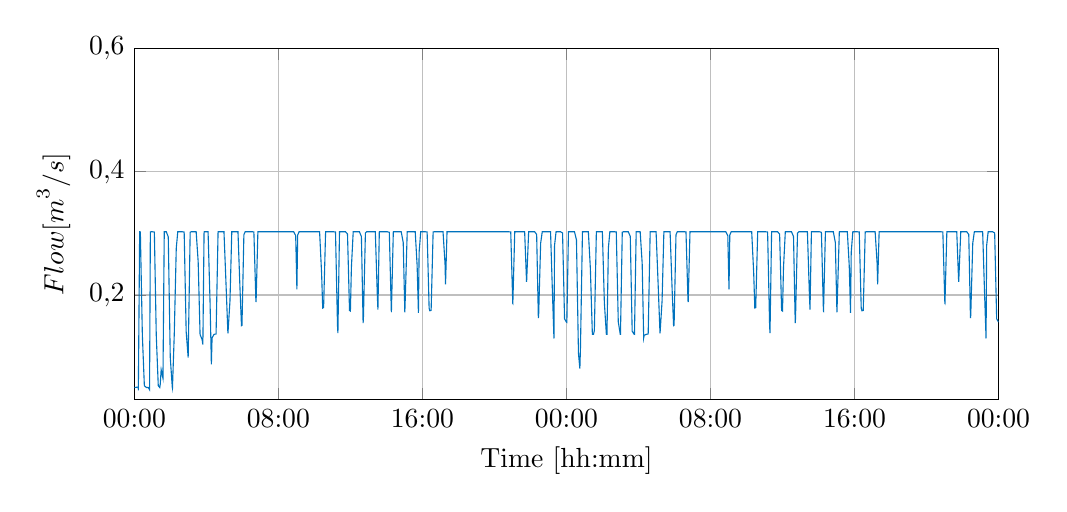
\begin{tikzpicture}

\begin{axis}[%
/pgf/number format/1000 sep={.},/pgf/number format/use comma,
width=4.321in,
height=1.7566in,
at={(0.758in,0.481in)},
scale only axis,
scaled x ticks = false,
xmin=1,
xmax=172801,
xtick={1,28801,57601,86401,115201,144001,172801},
xticklabels={{00:00},{08:00},{16:00},{00:00},{08:00},{16:00},{00:00},{},{},{}},
xlabel={Time [hh:mm]},
xmajorgrids,
ymin=0.03,
ymax=0.6,
ylabel={$\text{Flow [m}^\text{3}\text{/s]}$},
ymajorgrids,
axis background/.style={fill=white}
]
\addplot [color=mycolor1,solid,forget plot]
  table[row sep=crcr]{%
1	0.0499998683647933\\
41	0.049999868172035\\
781	0.0507074272387114\\
801	0.0453941788164327\\
1061	0.302680648501631\\
1201	0.302491862717989\\
1601	0.135010674602517\\
2001	0.052887199362477\\
2401	0.0500002155001922\\
2781	0.0499999795352394\\
3041	0.0464313962055376\\
3201	0.302516352986533\\
3361	0.302680760398885\\
3601	0.302680760242387\\
4001	0.302200169403778\\
4381	0.135164719879115\\
4781	0.0530325638925076\\
5081	0.0499386124360596\\
5181	0.055586808345944\\
5361	0.0789585569468111\\
5721	0.0650508632616179\\
5981	0.302680349454319\\
6061	0.302680760387634\\
6381	0.302680760225824\\
6781	0.294520901571626\\
7181	0.0989154154146933\\
7581	0.0506834888954093\\
7621	0.0489990780965182\\
7981	0.136213836996136\\
8381	0.275956670689325\\
8681	0.302680760374472\\
8761	0.302680760242582\\
8781	0.302680760242533\\
9161	0.302680760242539\\
9561	0.302680760242384\\
9961	0.302224863193897\\
10361	0.140899783082766\\
10761	0.0983633332953129\\
11161	0.301938752023508\\
11381	0.302680760374548\\
11561	0.302680760242539\\
12081	0.302680760242539\\
12361	0.302680758907861\\
12761	0.254130778077034\\
13141	0.136059459075788\\
13541	0.127963147712897\\
13701	0.119679046615807\\
13941	0.302599210033619\\
14121	0.302680760296439\\
14341	0.302680760242539\\
14741	0.302680311240456\\
15141	0.187225056092401\\
15401	0.0875542243229154\\
15541	0.130500480790875\\
15941	0.136229862037369\\
16341	0.136809631450867\\
16741	0.302680747416122\\
16781	0.302680760373209\\
17141	0.302680760242539\\
17521	0.302680760242539\\
17921	0.302680737957046\\
18321	0.219947517927539\\
18701	0.138590577002635\\
18721	0.138604494272073\\
19121	0.190596563317006\\
19481	0.302680760292888\\
19521	0.302680760240535\\
19541	0.302680760242636\\
19921	0.302680760242539\\
20061	0.302680760242539\\
20321	0.302680760242539\\
20721	0.302680667033518\\
21121	0.210941640765384\\
21421	0.150350637668172\\
21521	0.150919846322989\\
21901	0.297770119545691\\
22161	0.302680760321777\\
22341	0.302680760242539\\
22421	0.302680760242539\\
22821	0.302680760242539\\
23001	0.302680760242539\\
23101	0.302680760242539\\
23501	0.302680760242495\\
23901	0.302537137635991\\
24301	0.190721893188483\\
24341	0.188499862099904\\
24701	0.302674453583895\\
24841	0.302680760302086\\
25101	0.302680760242539\\
25121	0.302680760242539\\
25501	0.302680760242539\\
25761	0.302680760242539\\
25901	0.302680760242539\\
25921	0.302680760242539\\
26281	0.302680760242539\\
26401	0.302680760242539\\
26681	0.302680760242539\\
26721	0.302680760242539\\
27081	0.302680760242539\\
27201	0.302680760242539\\
27481	0.302680760242539\\
27521	0.302680760242539\\
27881	0.302680760242539\\
28001	0.302680760242539\\
28281	0.302680760242539\\
28321	0.302680760242539\\
28681	0.302680760242539\\
28801	0.302680760242539\\
29081	0.302680760242539\\
29121	0.302680760242539\\
29481	0.302680760242539\\
29601	0.302680760242539\\
29881	0.302680760242539\\
29921	0.302680760242539\\
30261	0.302680760242539\\
30401	0.302680760242539\\
30661	0.302680760242539\\
30721	0.302680760242539\\
31061	0.302680760242539\\
31201	0.302680760242539\\
31461	0.302680760242539\\
31861	0.302680760226753\\
32261	0.296420028519741\\
32501	0.209173907047401\\
32661	0.297306771900499\\
32941	0.302680760303886\\
33061	0.30268076024254\\
33121	0.302680760242539\\
33461	0.302680760242539\\
33541	0.302680760242539\\
33861	0.302680760242539\\
33881	0.302680760242539\\
34261	0.302680760242539\\
34341	0.302680760242539\\
34641	0.302680760242539\\
34661	0.302680760242539\\
35041	0.302680760242539\\
35141	0.302680760242539\\
35441	0.302680760242539\\
35461	0.302680760242539\\
35841	0.302680760242539\\
35941	0.302680760242539\\
36241	0.302680760242539\\
36261	0.302680760242539\\
36641	0.302680760242539\\
37041	0.302680753339297\\
37441	0.235362546925594\\
37661	0.178862851273356\\
37841	0.179726721090916\\
38241	0.302679901182408\\
38341	0.302680760369674\\
38641	0.302680760242539\\
38681	0.302680760242539\\
39021	0.302680760242539\\
39161	0.302680760242539\\
39421	0.302680760242539\\
39821	0.302680760242383\\
40221	0.302246236787972\\
40621	0.150161908855395\\
40701	0.138355218094442\\
41021	0.302680505297797\\
41101	0.302680760397179\\
41421	0.302680760242539\\
41821	0.302680760242539\\
42221	0.302680760236874\\
42621	0.29896191150583\\
43021	0.175043157155675\\
43201	0.174045701145115\\
43401	0.245007839133707\\
43761	0.302680760291471\\
43801	0.302680760241942\\
43821	0.30268076024268\\
44201	0.302680760242539\\
44421	0.302680760242539\\
44601	0.302680760242539\\
45001	0.302680760225498\\
45401	0.294854689284065\\
45741	0.154597389404819\\
45801	0.161872632227415\\
46201	0.300594841800177\\
46461	0.302680760297433\\
46661	0.302680760242539\\
46741	0.30268076024254\\
47001	0.302680760242539\\
47121	0.302680760242539\\
47401	0.302680760242539\\
47781	0.302680760242539\\
48181	0.302679294473203\\
48581	0.200009228323768\\
48701	0.176389469603216\\
48981	0.302635857631507\\
49161	0.302680760302131\\
49441	0.30268076024254\\
49501	0.302680760242539\\
49781	0.302680760242539\\
49821	0.302680760242539\\
50181	0.302680760242539\\
50581	0.302680760241978\\
50981	0.301769350069738\\
51381	0.173914545017793\\
51401	0.173726233856688\\
51781	0.302680629822221\\
51861	0.302680760304468\\
52161	0.302680760242539\\
52201	0.302680760242539\\
52561	0.302680760242539\\
52681	0.302680760242539\\
52961	0.302680760242539\\
53361	0.302680760137084\\
53761	0.285344840884799\\
54081	0.171864139229676\\
54161	0.191627473023309\\
54561	0.302680760304719\\
54601	0.302680760241107\\
54961	0.302680760242539\\
55221	0.302680760242539\\
55361	0.302680760242539\\
55381	0.302680760242539\\
55761	0.302680760242539\\
56161	0.302680753775212\\
56541	0.248103693023625\\
56801	0.171074960948495\\
56941	0.269357952492251\\
57261	0.302680760382393\\
57361	0.302680760242545\\
57381	0.302680760242537\\
57741	0.302680760242539\\
58141	0.302680760242382\\
58541	0.302295171065643\\
58941	0.178519772866686\\
59081	0.174485379811156\\
59341	0.175023560243573\\
59741	0.302414323796332\\
59941	0.302680760295648\\
60141	0.302680760242539\\
60521	0.302680760242539\\
60921	0.302680760242539\\
61321	0.302680760242539\\
61721	0.302680757508409\\
62121	0.250916696674108\\
62221	0.217178049193355\\
62521	0.302678349363428\\
62641	0.302680760365995\\
62921	0.302680760242539\\
62941	0.302680760242539\\
63321	0.302680760242539\\
63701	0.302680760242539\\
63721	0.302680760242539\\
63861	0.302680760242539\\
64121	0.302680760242539\\
64181	0.302680760242539\\
64521	0.302680760242539\\
64661	0.302680760242539\\
64901	0.302680760242539\\
64981	0.302680760242539\\
65301	0.302680760242539\\
65321	0.302680760242539\\
65701	0.302680760242539\\
65781	0.302680760242539\\
66101	0.302680760242539\\
66121	0.302680760242539\\
66501	0.302680760242539\\
66581	0.302680760242539\\
66901	0.302680760242539\\
66921	0.302680760242539\\
67301	0.302680760242539\\
67381	0.302680760242539\\
67701	0.302680760242539\\
67721	0.302680760242539\\
68101	0.302680760242539\\
68181	0.302680760242539\\
68501	0.302680760242539\\
68521	0.302680760242539\\
68901	0.302680760242539\\
68981	0.302680760242539\\
69281	0.302680760242539\\
69301	0.302680760242539\\
69681	0.302680760242539\\
69781	0.302680760242539\\
70081	0.302680760242539\\
70101	0.302680760242539\\
70481	0.302680760242539\\
70581	0.302680760242539\\
70881	0.302680760242539\\
70901	0.302680760242539\\
71281	0.302680760242539\\
71381	0.302680760242539\\
71681	0.302680760242539\\
71701	0.302680760242539\\
72081	0.302680760242539\\
72181	0.302680760242539\\
72481	0.302680760242539\\
72501	0.302680760242539\\
72881	0.302680760242539\\
72981	0.302680760242539\\
73281	0.302680760242539\\
73301	0.302680760242539\\
73661	0.302680760242539\\
73781	0.302680760242539\\
74061	0.302680760242539\\
74101	0.302680760242539\\
74461	0.302680760242539\\
74861	0.302680760242361\\
75261	0.302311271184687\\
75661	0.18665919885132\\
75681	0.186377908093398\\
76061	0.302680540675553\\
76141	0.302680760381895\\
76461	0.302680760242539\\
76561	0.302680760242539\\
76861	0.302680760242539\\
76881	0.302680760242539\\
77261	0.302680760242539\\
77661	0.302680760242539\\
78041	0.302679346850995\\
78421	0.221375299721665\\
78441	0.222915673995048\\
78841	0.302680760370048\\
78881	0.302680760240669\\
79241	0.302680760242539\\
79341	0.302680760242539\\
79641	0.302680760242539\\
80041	0.302680760236529\\
80441	0.298307689135177\\
80781	0.162515690792454\\
80841	0.167267729521989\\
81241	0.28422427348192\\
81561	0.302680760284575\\
81641	0.302680760242527\\
81661	0.30268076024254\\
82041	0.302680760242539\\
82421	0.302680760242539\\
82841	0.302680760242539\\
83221	0.302680350128537\\
83621	0.198122368841399\\
83901	0.129520173009044\\
84021	0.280726131825289\\
84321	0.302680760283294\\
84421	0.302680760242541\\
84501	0.302680760242539\\
84961	0.302680760242539\\
85221	0.302680760240646\\
85621	0.300661703676257\\
86021	0.161380700503718\\
86401	0.155964429214595\\
86481	0.155582157734116\\
86801	0.30264576683554\\
86961	0.302680760323372\\
87201	0.302680760242539\\
87221	0.302680760242539\\
87601	0.302680760242539\\
88001	0.302680760196296\\
88401	0.289554341303737\\
88801	0.105352012864476\\
89081	0.0805055894204873\\
89201	0.114306544292461\\
89601	0.302680564793237\\
89681	0.302680760369047\\
90101	0.302680760242539\\
90301	0.302680760242539\\
90401	0.302680760242539\\
90781	0.302680757285747\\
91181	0.243263335017434\\
91581	0.136340341814795\\
91801	0.136217239567303\\
91981	0.142512616322006\\
92381	0.302680760374472\\
92421	0.302680760241047\\
92781	0.302680760242539\\
93181	0.302680760242539\\
93581	0.302679090957024\\
93981	0.187376244627345\\
94381	0.136220528223306\\
94501	0.136217239567303\\
94781	0.275956670689325\\
95081	0.302680760374472\\
95161	0.302680760242582\\
95181	0.302680760242533\\
95561	0.302680760242539\\
95961	0.302680760242503\\
96361	0.302507962825889\\
96761	0.156582670700064\\
97161	0.136217322878085\\
97201	0.136217239567303\\
97561	0.301940416259168\\
97781	0.302680760374472\\
97961	0.302680760242539\\
98061	0.302680760242539\\
98361	0.302680760242539\\
98761	0.302680760226408\\
99161	0.295215417760891\\
99541	0.141416696559254\\
99941	0.136193758336533\\
100001	0.13614720808987\\
100341	0.302668105269287\\
100481	0.302680760332779\\
100741	0.302680760242539\\
101141	0.302680758864867\\
101541	0.251403371417926\\
101841	0.130500860209357\\
101941	0.134587291476283\\
102341	0.136229862445542\\
102741	0.136809631450867\\
103141	0.302680747416122\\
103181	0.302680760373208\\
103541	0.302680760242539\\
103921	0.302680760242539\\
104321	0.302680737957046\\
104721	0.219947517927539\\
105101	0.138590577002635\\
105121	0.138604494272073\\
105521	0.190596563317006\\
105881	0.302680760292888\\
105921	0.302680760240535\\
105941	0.302680760242636\\
106321	0.302680760242539\\
106461	0.302680760242539\\
106721	0.302680760242539\\
107121	0.302680667033518\\
107521	0.210941640765384\\
107821	0.150350637668172\\
107921	0.150919846322989\\
108301	0.297770119545691\\
108561	0.302680760321777\\
108741	0.302680760242539\\
108821	0.302680760242539\\
109221	0.302680760242539\\
109401	0.302680760242539\\
109501	0.302680760242539\\
109901	0.302680760242495\\
110301	0.302537137635991\\
110701	0.190721893188483\\
110741	0.188499862099904\\
111101	0.302674453583895\\
111241	0.302680760302086\\
111501	0.302680760242539\\
111521	0.302680760242539\\
111901	0.302680760242539\\
112161	0.302680760242539\\
112301	0.302680760242539\\
112321	0.302680760242539\\
112681	0.302680760242539\\
112801	0.302680760242539\\
113081	0.302680760242539\\
113121	0.302680760242539\\
113481	0.302680760242539\\
113601	0.302680760242539\\
113881	0.302680760242539\\
113921	0.302680760242539\\
114281	0.302680760242539\\
114401	0.302680760242539\\
114681	0.302680760242539\\
114721	0.302680760242539\\
115081	0.302680760242539\\
115201	0.302680760242539\\
115481	0.302680760242539\\
115521	0.302680760242539\\
115881	0.302680760242539\\
116001	0.302680760242539\\
116281	0.302680760242539\\
116321	0.302680760242539\\
116661	0.302680760242539\\
116801	0.302680760242539\\
117061	0.302680760242539\\
117121	0.302680760242539\\
117461	0.302680760242539\\
117601	0.302680760242539\\
117861	0.302680760242539\\
118261	0.302680760226753\\
118661	0.296420028519741\\
118901	0.209173907047401\\
119061	0.297306771900499\\
119341	0.302680760303886\\
119461	0.30268076024254\\
119521	0.302680760242539\\
119861	0.302680760242539\\
119941	0.302680760242539\\
120261	0.302680760242539\\
120281	0.302680760242539\\
120661	0.302680760242539\\
120741	0.302680760242539\\
121041	0.302680760242539\\
121061	0.302680760242539\\
121441	0.302680760242539\\
121541	0.302680760242539\\
121841	0.302680760242539\\
121861	0.302680760242539\\
122241	0.302680760242539\\
122341	0.302680760242539\\
122641	0.302680760242539\\
122661	0.302680760242539\\
123041	0.302680760242539\\
123441	0.302680753339297\\
123841	0.235362546925594\\
124061	0.178862851273356\\
124241	0.179726721090916\\
124641	0.302679901182408\\
124741	0.302680760369674\\
125041	0.302680760242539\\
125081	0.302680760242539\\
125421	0.302680760242539\\
125561	0.302680760242539\\
125821	0.302680760242539\\
126221	0.302680760242383\\
126621	0.302246236787972\\
127021	0.150161908855395\\
127101	0.138355218094442\\
127421	0.302680505297797\\
127501	0.302680760397179\\
127821	0.302680760242539\\
128221	0.302680760242539\\
128621	0.302680760236874\\
129021	0.29896191150583\\
129421	0.175043157155675\\
129601	0.174045701145115\\
129801	0.245007839133707\\
130161	0.302680760291471\\
130201	0.302680760241942\\
130221	0.30268076024268\\
130601	0.302680760242539\\
130821	0.302680760242539\\
131001	0.302680760242539\\
131401	0.302680760225498\\
131801	0.294854689284065\\
132141	0.154597389404819\\
132201	0.161872632227415\\
132601	0.300594841800177\\
132861	0.302680760297433\\
133061	0.302680760242539\\
133141	0.30268076024254\\
133401	0.302680760242539\\
133521	0.302680760242539\\
133801	0.302680760242539\\
134181	0.302680760242539\\
134581	0.302679294473203\\
134981	0.200009228323768\\
135101	0.176389469603216\\
135381	0.302635857631507\\
135561	0.302680760302131\\
135841	0.30268076024254\\
135901	0.302680760242539\\
136181	0.302680760242539\\
136221	0.302680760242539\\
136581	0.302680760242539\\
136981	0.302680760241978\\
137381	0.301769350069738\\
137781	0.173914545017793\\
137801	0.173726233856688\\
138181	0.302680629822221\\
138261	0.302680760304468\\
138561	0.302680760242539\\
138601	0.302680760242539\\
138961	0.302680760242539\\
139081	0.302680760242539\\
139361	0.302680760242539\\
139761	0.302680760137084\\
140161	0.285344840884799\\
140481	0.171864139229676\\
140561	0.191627473023309\\
140961	0.302680760304719\\
141001	0.302680760241107\\
141361	0.302680760242539\\
141621	0.302680760242539\\
141761	0.302680760242539\\
141781	0.302680760242539\\
142161	0.302680760242539\\
142561	0.302680753775212\\
142941	0.248103693023625\\
143201	0.171074960948495\\
143341	0.269357952492251\\
143661	0.302680760382393\\
143761	0.302680760242545\\
143781	0.302680760242537\\
144141	0.302680760242539\\
144541	0.302680760242382\\
144941	0.302295171065643\\
145341	0.178519772866686\\
145481	0.174485379811156\\
145741	0.175023560243573\\
146141	0.302414323796332\\
146341	0.302680760295648\\
146541	0.302680760242539\\
146921	0.302680760242539\\
147321	0.302680760242539\\
147721	0.302680760242539\\
148121	0.302680757508409\\
148521	0.250916696674108\\
148621	0.217178049193355\\
148921	0.302678349363428\\
149041	0.302680760365995\\
149321	0.302680760242539\\
149341	0.302680760242539\\
149721	0.302680760242539\\
150101	0.302680760242539\\
150121	0.302680760242539\\
150261	0.302680760242539\\
150521	0.302680760242539\\
150581	0.302680760242539\\
150921	0.302680760242539\\
151061	0.302680760242539\\
151301	0.302680760242539\\
151381	0.302680760242539\\
151701	0.302680760242539\\
151721	0.302680760242539\\
152101	0.302680760242539\\
152181	0.302680760242539\\
152501	0.302680760242539\\
152521	0.302680760242539\\
152901	0.302680760242539\\
152981	0.302680760242539\\
153301	0.302680760242539\\
153321	0.302680760242539\\
153701	0.302680760242539\\
153781	0.302680760242539\\
154101	0.302680760242539\\
154121	0.302680760242539\\
154501	0.302680760242539\\
154581	0.302680760242539\\
154901	0.302680760242539\\
154921	0.302680760242539\\
155301	0.302680760242539\\
155381	0.302680760242539\\
155681	0.302680760242539\\
155701	0.302680760242539\\
156081	0.302680760242539\\
156181	0.302680760242539\\
156481	0.302680760242539\\
156501	0.302680760242539\\
156881	0.302680760242539\\
156981	0.302680760242539\\
157281	0.302680760242539\\
157301	0.302680760242539\\
157681	0.302680760242539\\
157781	0.302680760242539\\
158081	0.302680760242539\\
158101	0.302680760242539\\
158481	0.302680760242539\\
158581	0.302680760242539\\
158881	0.302680760242539\\
158901	0.302680760242539\\
159281	0.302680760242539\\
159381	0.302680760242539\\
159681	0.302680760242539\\
159701	0.302680760242539\\
160061	0.302680760242539\\
160181	0.302680760242539\\
160461	0.302680760242539\\
160501	0.302680760242539\\
160861	0.302680760242539\\
161261	0.302680760242361\\
161661	0.302311271184687\\
162061	0.18665919885132\\
162081	0.186377908093398\\
162461	0.302680540675553\\
162541	0.302680760381895\\
162861	0.302680760242539\\
162961	0.302680760242539\\
163261	0.302680760242539\\
163281	0.302680760242539\\
163661	0.302680760242539\\
164061	0.302680760242539\\
164441	0.302679346850995\\
164821	0.221375299721665\\
164841	0.222915673995048\\
165241	0.302680760370048\\
165281	0.302680760240669\\
165641	0.302680760242539\\
165741	0.302680760242539\\
166041	0.302680760242539\\
166441	0.302680760236529\\
166841	0.298307689135177\\
167181	0.162515690792454\\
167241	0.167267729521989\\
167641	0.28422427348192\\
167961	0.302680760284575\\
168041	0.302680760242527\\
168061	0.30268076024254\\
168441	0.302680760242539\\
168821	0.302680760242539\\
169241	0.302680760242539\\
169621	0.302680350128537\\
170021	0.198122368841399\\
170301	0.129520173009044\\
170421	0.280726131825289\\
170721	0.302680760283294\\
170821	0.302680760242541\\
170901	0.302680760242539\\
171361	0.302680760242539\\
171621	0.302680760240646\\
172021	0.300661703676257\\
172421	0.161380700503718\\
172801	0.155964429214595\\
};
\end{axis}
\end{tikzpicture}%
\caption{Output of the last pipe in to the WWTP, where a tank has been placed in front to smooth out the flow.}
\label{fig:simulation_output_second}
\end{figure} 

tank spec, size=  300 , height =5,	area=60
			   